\chapter{Learning Symbolic Representations over Time}
\label{chap:kandycem}


In this chapter we consider a learning setting where Neural Networks have to develop autonomously novel concepts, possibly organized into a hierarchy, capable of aiding predictions on some high-level tasks.
For example, consider the problem of predicting whether an input pattern belongs to category ``cat'', which an agent is required to solve as a function of its concept-level predictions. %Suppose that the agent takes 
The agent can take a positive decision, not only because of a fully black-box process, but because it also predicts the concepts ``fur'', ``tail'', ``paws'', and the absence of ``engine'' or ``wheels''. This setting improves explainability and control (concepts could also be artificially manipulated, if needed), and corresponds to the one of Concept Bottleneck Models.
Concept-level annotations are, however, an expensive source of knowledge in virtue of their density. At the same time, human learners are equipped with the ability of grasping novel concepts in a goal-oriented manner (e.g., when learning to perform a novel task, by means of teacher-student demonstrations, a human student can independently distill a ``toolbox'' of concepts which are beneficial for the task at hand, while relying on the teacher's guidance only sporadically).
Locatello et al.~\cite{locatello2019challenging} provided strong theoretical and practical arguments against the successful disentanglement of concepts in fully unsupervised settings, unless the learning agent is equipped with strong priors.
At the same time, curriculum learning is a natural form of human training, which can also be employed in Machine Learning to improve generalization~\cite{bengio2009curriculum}.
In this chapter we explore whether time, in the form of a curricular progression of binary classification tasks, can be a suitable prior for \textit{unsupervised} concept disentanglement.
The content of this chapter is adapted from our CoLLAs 2024 conference paper~\cite{lorello2024continual}.

\section{Background}
Humans naturally discover new concepts through time, without the need of ``supervision''. This is especially true in child development, during which autonomous exploration leads to concept formation~\cite{damon2008child}, but remains a relevant form of learning also for adults.
%Discovering concepts through time is a natural way of learning in humans, and especially in children~\cite{damon2008child}, where ``supervisions'' are limited. 
In the case of machines, unsupervised concept discovery intrinsically requires suitable inductive biases~\cite{locatello2019challenging}. Incrementally disclosing concepts over time is not only aligned with what happens in humans, but it can also provide precious information for Machine Learning purposes, capable of guiding discovery along a sequence of smaller, but feasible, steps, aimed at building a vocabulary of concepts relevant for a specific domain.
This opportunity is traded-off by the additional challenge of preventing catastrophic forgetting, not only at the task level, but also at the concept level~\cite{marconato2023neuro}, while also preserving the plasticity required to update wrongly identified concepts. Such a challenging, yet important, scenario is largely overlooked in the literature.
%
The vast majority of approaches to concept learning, in fact, strongly relies on supervisions, that must be specifically provided not only at the level of tasks, but also at the level of concepts.
%
%As a notable example, Concept Bottleneck Models (CBMs)~\cite{koh2020concept} have been recently introduced as an interpretable model that learns from the input an intermediate layer of concepts, upon which classification is performed. While Boolean CBMs exploit a hard activation function (i.e., a threshold) to enable concept triggering, Fuzzy CBMs use a soft activation (e.g., a sigmoid) to enhance the expressive power of the model, even though at the cost of a lower interpretability. %In both cases, CBMs are fully supervised at the level of concepts, which means that training examples have to be annotated with concept information. 
%The need of full task-level and concept-level supervisions has been partially relaxed in Hybrid CBMs~\cite{mahinpei2021promises}, based on a combination of both supervised and unsupervised concepts to give the model some additional degrees of freedom.
%
%As an expansion of CBMs, Concept Embeddings Models (CEMs)~\cite{espinosa2022concept} extend the representation of each concept with two embeddings that are associated to the active and inactive state of the concept, respectively.
%
Some attempts to perform unsupervised learning of disentangled representations, that can be associated to low-level visual concepts, have been recently inspired by neuroscience~\cite{higgins2016early}, using a generative model implemented via variational auto-encoders, whose learning is driven by principles that mimic the ventral visual stream in our brain.
%
On a different perspective, a first attempt of exploiting semi-supervised concept learning in a Continual Learning setting has been proposed by Marconato et al.~\cite{marconato2023neuro}, who focus on a Neuro-symbolic scenario where domain background knowledge is available, and it is exploited to consolidate concept learning with supervisions across a sequence of tasks. The problem is addressed by modeling the conditional probability distribution of concepts with respect to the input data, and by enforcing the stability of such probability distribution through time. The approach is coupled with a Neuro-symbolic system, where background knowledge is exploited to drive learning and avoid reasoning shortcuts.

\section{Methodology}
\label{cem:sec:method}
We focus on a teacher-student scenario where the teacher presents the student with samples of a sequence of $N$ binary tasks, considered appropriate to improve the student understanding skills. %The teacher proposes a sequence of $|\mathcal{T}|$ binary tasks, with the 
The student is expected to get better at discriminating examples of the selected tasks and also to progressively acquire an improved representation of the world, developing, reusing and mixing latent concepts to solve each task. These concepts are not made explicit, thus no supervision is given about them.
Data is provided to the learning agent (student) through a potentially lifelong stream where, at each time instant $t$, a small batch of samples $\sX^{(t)}$ (from a certain task) is made available, together with their task-id and their task-level labels $\sY^{(t)}$. Concept labels $\sC$ are never exposed to the agent, but their ground truth will be used to assess the quality of autonomously developed concepts. 
The agent is aware of task switches, thus we are in a Task-incremental setting~\cite{van2022three}.
%
The issues with this setting are not only those typical of Continual Learning, such as catastrophic forgetting~\cite{parisi2019continual} at the task-level, but also internal stability issues that might lead to concept drift~\cite{marconato2023neuro}. As a matter of fact, even if the set of concepts $\sC$ is not defined in advance (and, in general, it is not known at all), the agent must avoid forgetting previously developed concepts. %, if they had been helpful in solving older tasks. 
The agent is also expected to learn how to compose the already stable concepts with newly discovered ones.
%
We propose to tackle this scenario introducing specific criteria to constrain the Neural Network in order to (i.) \textit{favour the development of %either strongly active or strongly inactive concepts, 
strongly polarized concept activations}, (ii.) \textit{increase the correlation between tuples of concepts and tasks}, (iii.) \textit{progressively promote stability over time}. The first requirement is fundamental in concept-based learning, since it makes it easy to take a crisp decision on the state of each concept $j$ given its dense activation $\evc_j$, promoting interpretability. The second requirement ensures the presence of an inductive bias linking the final task with a subset of active/inactive concepts, ensuring that the agent is profitably learning to organize its internal knowledge. The final requirement is typical of Continual Learning, to discourage catastrophic forgetting, %even if, in this case, it applies also 
in this case also with respect to concepts, which are unsupervised and not completely learned during the first tasks, but that are expected to develop during the life of the agent.

\paragraph{Hamming Triplet Loss.} 
 %When supervision is available at a concept level, fuzzy concept bottlenecks can be effectively trained once each $c_i$ is interpreted as a probability score associated to concept activation. %  have been interpreted as probability vectors, which, in the supervised case, allows straight-forward training. % , by means of cross-entropy.
%However, in the case of this paper, supervisions are only available at a task level, and ground truth concepts distributions are not given, 
To counteract the lack of extra knowledge on the problem and on the ground truth concepts distribution, we propose an interpretation of concepts based on a perspective that intersects notions behind Deep Hashing~\cite{luo2023survey}: discretized concept vectors $\hat{\vc}$ can be considered binary hashes, which partition the input space in a way that promotes collisions between semantically similar (i.e., associated to the same task label) samples.
%
This interpretation allows us to define a straightforward Distance Metric Learning approach based on the Hamming distance, in the form of a continuous and differentiable relaxation %which is not based on binary vectors, but 
%based on the
exploiting the $\normlone$ norm applied to pairs of concept vectors: 
\begin{equation*}
	D_{H}(\vc_i, \vc_j) = \| \vc_i - \vc_j \|_1.
	%\label{cem:eq:l1}
\end{equation*}
The Metric Learning problem is handled by comparing triples of input patterns, as typical in the popular Triplet Loss framework~\cite{dong2018triplet}. For each task $f^{(t)}: \sX^{(t} \mapsto \sY^{(t)}$, a triple is composed of the concept activation vectors ($\vc$) (i.) of an {\it anchor} sample, (ii.) of a sample with the same task-level label of the anchor (i.e., task-positive or task-negative, named {\it positive} element of the triple), and (iii.) a third example with opposite task-level label (i.e., task-negative or task-positive, respectively -- named {\it negative} element). Minimizing the Triplet Loss favors the development of similar concept vectors for examples with the same label, and different vectors for pairs with different labels. It is important to remark that, within each task, examples with the same task-level label are expected to share some concepts (the ones that are relevant for the considered task), while there is no need to force coherence on the remaining ones. For this reason, the criterion we propose must be interpreted as a soft regularizer and not as a strongly enforced constraint.
%
%In detail, within each mini-batch from the data stream, 
We build a set of triples performing Semi-hard Negative Mining~\cite{schroff2015facenet} on mini-batches of the dataset. 
Plugging the (relaxed) Hamming distance in a Triplet Loss with margin $\mu$, we get the Hamming triplet loss $\mathcal{L}_H$:\footnote{If no triples can be mined within the mini-batch, the loss assumes a default value of 0.} 
\begin{equation*}
	%d^h(\vx, \vy) = \normlone(\vx - \vy)\\
	\mathcal{L}_H\left(\langle\mC_A, \mC_P, \mC_N\rangle, \mu\right) = \sum_{i = 0}^{N-1} \left(\|\mC_A[i,:], \mC_P[i,:]\|_1 - \|\mC_A[i,:], \mC_N[i,:]\|_1 + \mu\right)^+,
	%\label{cem:eq:triplet}
\end{equation*}
where $\mC_A[i,:], \mC_P[i,:], \mC_N[i,:]$ are the concept vectors of the $i$-th anchor, positive and negative samples, respectively, of the batch of triples.
%being $A_i$, $P_i$, $N_t$ the $i$-th elements of the respective collections. 
The margin hyper-parameter $\mu$ assumes an intuitive interpretation, corresponding to the expected minimum ``concept-distance'' between positive and negative samples.
%which is expected between pairs of concept activations of any positive-negative pair.

%\vspace{-1mm}
\paragraph{Concept Replay.} Enforcing $\mathcal{L}_H$ is not enough to guarantee stability on the learned concepts, that might incur in non-predictable dynamics over time. For this reason, we developed a novel replay strategy, based on an augmented replay buffer which is used both for experience replay at the level of task objective and as feature replay at the concept level. The replay buffer is governed by a Class-balanced Reservoir Sampling~\cite{chrysakis2020online} policy, and it memorizes, for each input sample, both the given task-level label and the binarized concept representation $\hat{\vc}$.
%
Concept replay is implemented as a second round of Hamming Triplet Loss, exploiting the buffered concepts. Since the buffer $\gB$ contains data from (a subset of) the tasks seen so far, we mine a mini-batch of triples for each of them, by means of a uniform sampling strategy. %We indicate with $\xi_{\mathcal{U}}(B_X, B_Y, B_C)$ the triplet mining function, which is different from the already introduced $\xi_{\mathcal{SH}}(X,Y)$ for the following reasons. 
The anchor samples, taken from $\gB_X$, are fed to the net, computing fresh concept representations $\vc$'s, while the concept vectors for the positive and negative samples of the triples are directly retrieved from $\gB_{C}$, thus they are binary vectors.\footnote{Since data from the current task is directly provided to the network (i.e., it comes from the input stream), the anchors of the triples for the current task are sampled from $\sX^{(t)}$. We avoid making this explicit, to keep the notation simple.} Such binary vectors act as constant and polarized targets. Hence, when minimizing the Triplet Loss, only the concept activations of the anchors are altered, pushing them toward (resp. far away from) the constant binary targets of the positive (resp. negative) elements. As a result, buffered binary concepts implicitly help polarize the learned concept probabilities towards 0 or 1, and they are more storage efficient, which is a crucial property to limit the memory used by the buffered samples. In order to avoid aging of the binary concepts in $\gB_{C}$, at the end of each epoch $\gB_{C}$ is recomputed from scratch.

\paragraph{Aggregated Loss Function.} Let $\langle\sX^{(t)}, \sY^{(t)}\rangle$ be a fresh mini-batch from the current dataset, $\langle\gB_X, \gB_Y, \gB_C\rangle$ a mini-batch sampled from the replay buffer, $\xi_{SH}$ the Semi-hard Negative Mining function, and $\xi_{U}$ the Uniform Mining function, then the total loss function $\mathcal{L}$ is the sum of four contributions:\footnote{The Mining functions $\xi_\cdot$ return mini-batches $\langle\mC_A, \mC_P, \mC_N\rangle$ of triples in concept space.}
\begin{align*}
	\mathcal{L}(\langle \sX^{(t)}, \sY^{(t)}, \gB_X, \gB_Y, \gB_C \rangle) =&  \mathcal{L}_{\mathrm{BCE}}\left(\sX^{(t)}, \sY^{(t)}\right) + \\
	& \lambda_r \cdot \mathcal{L}_{\mathrm{BCE}}\left(\gB_X, \gB_Y\right) + \\
	&\frac{\lambda_h}{2} \cdot \mathcal{L}_H\left(\xi_{SH}\left(\sX^{(t)}, \sY^{(t)}\right), \mu\right) +\\
	&\frac{\lambda_h}{2} \cdot \mathcal{L}_{H}\left(\xi_{U}\left(\gB_X, \gB_Y, \gB_C\right), \mu\right).
	\label{cem:eq:loss}  
\end{align*}
The (i.) \textit{task-level loss} is a binary cross-entropy ($\mathcal{L}_{\mathrm{BCE}}$) applied to the batch of input data ($\sX$, $\sY$). (ii.) \textit{Task-level experience replay} is based on the same loss, applied however to buffered data ($\gB_X$, $\gB_Y$) and weighted by $\lambda_r > 0$. Finally, the contrastive term, weighted by $\lambda_h > 0$, is the average of the \textit{Hamming Triplet Loss} applied to (iii.) input and (iv.) buffered samples.

\begin{figure}
	\centering
	\begin{subfigure}{.21\textwidth}
		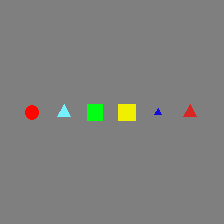
\includegraphics[width=\textwidth]{imgs/cem/KANDY_1-T12-pos.png}
		\caption{}%KANDY 1 POSITIVE (TASK 12, red triangle on right + blue at any position)}
\end{subfigure}
\begin{subfigure}{.21\textwidth}
	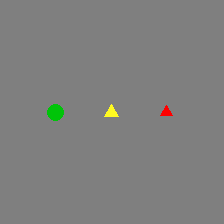
\includegraphics[width=\textwidth]{imgs/cem/KANDY_1-T12-neg.png}
	\caption{}%KANDY 1 NEGATIVE (TASK 12)}
\end{subfigure}
\hfill
\begin{subfigure}{.21\textwidth}
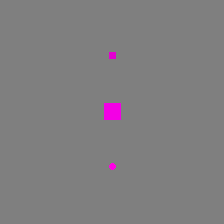
\includegraphics[width=\textwidth]{imgs/cem/KANDY_2-T24-pos.png}
\caption{}%KANDY 2 POSITIVE (TASK 24, shared attribute)}
\end{subfigure}
\begin{subfigure}{.21\textwidth}
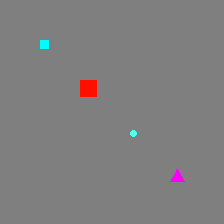
\includegraphics[width=\textwidth]{imgs/cem/KANDY_2-T24-neg.png}
\caption{}%KANDY 2 NEGATIVE (TASK 24)}
\end{subfigure}
%\vskip -3mm
\caption[Examples from KANDY]{Task examples. Left: positive (a) and negative (b) examples for task 12 in KANDY-1, positive class being defined by a red triangle on the right, plus the presence of a blue object anywhere. Right: positive (c) and negative (d) examples for task 24 in KANDY-2, positive class being defined by objects that share one attribute (in this case, color).
%\vspace{-4mm}
}
\label{cem:fig:kandy-examples}
\end{figure}


\section{Experiments}\label{cem:sec:experiments}
The experimental setup follows the one described in Section~\ref{sec:kandy:neur-exp}, with some differences. Namely, we employ the same (ii.) \textsc{CNN}, (iv.) \textsc{ResNet-50 (H)} and (v.) \textsc{ViT-16 (H)} backbones, and compare the (ii.) \textit{Joint} and (iii.) \textit{Task-incremental} learning settings.
In contrast with the experiments on \textsc{KANDY-Induction}, the output of neural backbones $\phi_\vtheta: \sX \mapsto \R^d$ is fed to a Concept Embedding Model $\psi_{\vtheta'}: \R^d \mapsto \R^e \times \R^e$, and then to the final binary classification head $\omega^{(t)}_{\vtheta"}: \R^{2\cdot e} \mapsto [0, 1]$.\footnote{As in the case of \textsc{KANDY-Induction} experiments, there is a different binary classifier for each task in the curriculum.}
The Concept Embedding Layer is characterized by 30 concepts (larger than the number of ground truth concepts in \textsc{KANDY-Concepts-1} and \textsc{KANDY-Concepts-2}). The linear mappings $\rho^{pos}$, $\rho^{neg}$, within the Concept Embedding Layer, produce 12-dimensional embeddings and share parameters across every concept, following the original implementation~\cite{espinosa2022concept}, embeddings are then collapsed to concept logits and then normalized in the $[0, 1]$ range by means of a sigmoid non-linearity.
Concept-only metrics are computed on concept logits, probed before the sigmoid activation.
The proposed concept replay strategy is applied only on the \textit{Task-incremental} setting, while the proposed Hamming Triplet Loss is applied to both learning settings.
In the Task-incremental setting, each task is trained sequentially, shuffling data points within the task, while the Joint setting is characterized by a global shuffling prior to each epoch. The optimization steps are equivalent in both cases (each task is trained for 10 epochs before moving to the next in the Task-incremental setting, while the Joint setting is trained for 10 global epochs).


\paragraph{Hyper-parameters.} Our experimental activity is aimed at validating the role of the proposed learning criteria. For this reason, we evaluated different values of $\lambda_r$, $\lambda_t$, $\mu$, accordingly to the following grids, which were selected after an initial set of preliminary experiments: $\lambda_r \in \{ 0, 1, 10 \}$, $\lambda_t \in \{ 0, 1, 10 \}$, $\mu = \{ 1, 4 \}$. We also considered a replay buffer of size $200$,\footnote{This amount (corresponding to $9\%$ and $4\%$ of the total number of samples for each dataset, respectively) is small enough not to bias evaluation in favor of the Continual Learning setting, compared to the Joint one.} Adam optimizer with learning rate set to $0.001$, batch size $|\sX^{(t)}|$ = $32$.
%We fix the following hyper-parameters: $\text{buffer\_size} = 200$, $\text{learning\_rate} = 0.001$ (Adam), $\text{batch\_size} = 32$, $\text{n\_concepts} = 30$, $\text{cem\_emb\_size} = 12$.
%Variable hyper-parameters in our experiments are: $\lambda_r = [0, 1.0, 10.0], \lambda_t = [0, 1.0, 10.0], m = [1, 4], \text{model} = [\text{cnn}, \text{ResNet-50}, \text{vit}], \text{training\_regime} = [\text{joint}, \text{continual\_task\_incremental}]$.
During training we performed the following image augmentation operations: random rotation, random resize crop, normalization. %At evaluation, we only perform normalization.
Although datasets have a negligible imbalance between task-positive and task-negative samples, we ensured batches to be balanced. %Similarly, when storing new elements in the replay buffer, we used a Balanced Reservoir Sampling strategy~\cite{kim2020imbalanced}. 

\paragraph{Validation.} In the Joint learning setting, the optimal values of the hyperparameters were found by maximizing the accuracy of the validation set. For the Task-incremental case, we followed the more challenging and realistic setting in which only some initial tasks are used for validation purposes, considering that the learning horizon is virtually lifelong. This can be perfectly simulated in  the proposed datasets, %. In fact, tasks are organized in a way which encourages learning of concepts in a structured way, 
which presents basic concepts first, and then, in the later tasks, combines them for more advanced problems. This allowed us to %take a clear decision on the proper time in which model selection should be performed, considering specific task boundaries which correspond to 
unambiguously identify the last task in which a new basic/ground truth concept is introduced (task 8 in \textsc{KANDY-Concepts-1} and the end of task 17  in \textsc{KANDY-Concepts-2}), and the subsequent task are excluded from the validation procedure.\footnote{This idea is inspired by human education, in which a teacher is well aware, not only of the optimal order in which topics should be presented to students, but also at which point should their performance be evaluated for the best diagnosis of the learning process.} This choice makes the Task-incremental learning experience even more challenging when compared to the Joint case, where validation data from all the tasks is available. All the results of this chapter refer to the test sets, using the best model found with the described validation criterion.

\paragraph{Task-related Metrics.} Similar to Section~\ref{sec:kandy:neur-exp}, we consider \textsc{\small Average Accuracy} and \textsc{\small Average Forgetting} as main metrics.\footnote{We also measured forward/backward transfer, that we found to be not significantly pronounced, thus we avoid reporting them.} Additionally, in order to evaluate the way tuples of concepts are aligned to tasks, we considered what we refer to as {\sc\small Task Alignment Score} ({\small\sc TAS}). This score is a direct transposition of the alignment measure considered when evaluating Concept Embedding Models~\cite{espinosa2022concept}, which is named {\sc\small Concept Alignment Score} ({\small\sc CAS}) in their work. The original implementation assumed supervised concepts, and the goal was to measure the alignment of each concept embedding in relation to the supervised concept it represented. In the context of this chapter, however, we are interested instead in measuring the alignment of concept activation scores $\vc$ and each task in the curriculum.\footnote{We reused the code of~\cite{espinosa2022concept}, using the concept logit vector prior the sigmoid functions that yields $\vc$.}

\paragraph{Concept-only Metrics.} When restricting the evaluation to the concept bottleneck only, our goal is to evaluate how similar are the discovered concepts to the ground truth concepts annotations. We considered four different measures. The first one is another instance of the already introduced {\small\sc Concept Alignment Score}, in this case named {\sc\small Ground Concept Alignment Score} ({\small\sc GCAS}), which measures the averaged (over ground truth concepts) alignment of concept activation scores $\vc$ and each (expected) ground truth concept. 
%
The second and third metrics are based on the correlation matrices between ground truth concepts and discovered concepts, and vice-versa, respectively. In particular, we computed the {\sc\small Matthews Correlation Coefficient} ({\sc\small MCC})~\cite{matthews1975comparison} for each entry of the two matrices. Differently from {\small\sc GCAS}, here we focus on binarized concepts $\hat{\vc}$. We aggregate the results on each matrix by means of the  {\sc\small Jensen-Shannon divergence}~\cite{menendez1997jensen} ({\small\sc JSD}), either normalizing rows (i.e., with respect to true concepts, {\small\sc JSD-T}) or column (i.e., with respect to predicted concepts, {\small\sc JSD-P}) to probability distributions. %considering each normalized row as a probability distribution describing how likely it is for a predicted concept to be mapped to each of the ground truth concepts ({\small\sc JSD-T}), or considering each normalized column as a probability distribution describing how likely it is for a ground truth concept to be represented by each of the predicted concepts ({\small\sc JSD-P}). 
In the former case, intuitively, we penalize predicted concepts which allocate probability to more than one true concept, while in the latter we penalize redundant representations of true concepts.
The last metric we propose focuses on comparing the correlation between predicted concepts and themselves. The entries of the {\sc\small MCC}-based correlation matrix are aggregated into the so-called {\small\sc Diagonalization Score} ({\small\sc DIAGS}), that measures how close is the correlation matrix to a diagonal matrix, where concepts are encoding independent aspects (the larger the better).
Appendix~\ref{app:kandycemmetrics} contains an extended definition of the proposed metrics.


\section{Results}

\paragraph{Tasks vs. Concepts.} Table~\ref{cem:tab:main} reports our main experimental results. We compare {\small\sc Average Accuracy} and {\small\sc TAS} in the Task-incremental and Joint learning cases. 
Overall differences in {\small\sc Average Accuracy} are not significant. Accuracy is slightly larger in the Task-incremental setting for \textsc{KANDY-Concepts-1}, while it is slightly larger in the Joint setting for \textsc{KANDY-Concepts-2}. 
%
The main focus of this experiment consists in evaluating the properties of discovered concepts. We observe how the Task-incremental setting consistently achieves significantly better results in terms of {\small\sc TAS} for both datasets, indicating that discovery over time yields concept representations that are more aligned with tasks. This behavior is consistent across every considered backbone.
The proposed concept-level triplet loss is not, alone, sufficient to boost task-alignment. This claim is sustained by the fact that the Joint learning setting (which is also using the triplet loss) is producing concepts which are significantly less aligned with respect to the tasks.
%We remark that also the Joint training case is exploiting the proposed concept-level triplet loss, thus the just described result is mostly due to the role of the concept replay, that helps in stabilizing the concept layer when learning in a continual manner.
 %Moreover, this happens independently on the considered neural architectures.
In order to better evaluate this result we performed an ablation study to analyze the impact of the triplet loss on concept learning: we report the value of {\small\sc TAS} for this experiment in Figure~\ref{cem:fig:tas-ablation}. Results show that discarding the triplet loss yields a significant drop in performance for both \textsc{ResNet-50} and \textsc{ViT-16} models in the Task-incremental setting, especially on the \textsc{KANDY-Concepts-2} dataset. The \textsc{CNN} model is almost unaffected, this might be due to the cold start of the training procedure, as concepts that are badly developed in the early stages of life of the agent, end up in being stored in the replay buffer, and they tend to push the network toward potentially sub-optimal configurations. This suggest that there might be room for schemes that progressively enforce the triplet loss and concept replays. In the Joint learning setting (Figure~\ref{cem:fig:tas-ablation}), the impact of the triplet loss is less evident, suggesting that it is the combined effect of our concept-level loss and of a progressive learning setting that favors the development of concepts that better encode the task properties.


\begin{table}
%\vskip -10mm
\centering
\resizebox{\textwidth}{!}{\begin{tabular}{cccccc}
\toprule
\multirow{2}{*}{\sc Model} & \multirow{2}{*}{\sc Setting} & \multicolumn{2}{c}{{\small\sc KANDY-Concepts-1}} & \multicolumn{2}{c}{{\small\sc KANDY-Concepts-2}} \\
\cmidrule{3-6}
%\rowcolor{Gray}
& & {\small\multirow{2}{*}{\shortstack[c]{\sc Average\\\sc Accuracy}} \raisebox{-1.5ex}{\:$\uparrow$}} & \multirow{2}{*}{\small\sc \underline{TAS} $\uparrow$} & {\small\multirow{2}{*}{\shortstack[c]{\sc Average\\\sc Accuracy}} \raisebox{-1.5ex}{\:$\uparrow$}} & \multirow{2}{*}{\small\sc \underline{TAS} $\uparrow$} \\
& & & & & \\
\midrule
%\multicolumn{4}{c}{CNN}\\
%\multirow{2}{*}{CNN}& Continual & \cellcolor{Gray}{0.65 $$ {\tiny ($\pm 0.02$)}} & \cellcolor{Gray}{\bf 0.79 $$ {\tiny ($\pm 0.01$)}} & \cellcolor{Gray}0.69 $$ {\tiny ($\pm 0.03$)} & \cellcolor{Gray}{\bf 0.82 $$ {\tiny ($\pm 0.00$)}} \\
\multirow{2}{*}{CNN}& Task-incremental & {0.65 $$ {\tiny ($\pm 0.02$)}} & {\bf 0.79 $$ {\tiny ($\pm 0.01$)}} & 0.69 $$ {\tiny ($\pm 0.03$)} & {\bf 0.82 $$ {\tiny ($\pm 0.00$)}} \\
& Joint & 0.62 $$ {\tiny ($\pm 0.06$)} & 0.65 $$ {\tiny ($\pm 0.04$)} & {0.70 $$ {\tiny ($\pm 0.01$)}} & 0.50 $$ {\tiny ($\pm 0.03$)} \\
\hdashline
%\multicolumn{4}{c}{ResNet-50}\\
\multirow{2}{*}{ResNet-50}&
%Continual & \cellcolor{Gray}{0.73 $$ {\tiny ($\pm 0.01$)}} & \cellcolor{Gray}{\bf 0.76 $$ {\tiny ($\pm 0.01$)}} & \cellcolor{Gray}0.74 $$ {\tiny ($\pm 0.02$)} & \cellcolor{Gray}{\bf 0.78 $$ {\tiny ($\pm 0.02$)}} \\
Task-incremental & {0.73 $$ {\tiny ($\pm 0.01$)}} & {\bf 0.76 $$ {\tiny ($\pm 0.01$)}} & 0.74 $$ {\tiny ($\pm 0.02$)} & {\bf 0.78 $$ {\tiny ($\pm 0.02$)}} \\
& Joint & 0.70 $$ {\tiny ($\pm 0.02$)} & 0.68 $$ {\tiny ($\pm 0.07$)} & {0.79 $$ {\tiny ($\pm 0.02$)}} & 0.57 $$ {\tiny ($\pm 0.02$)} \\
\hdashline
\multirow{2}{*}{ViT-16}&
%\multicolumn{4}{c}{ViT}\\
%Continual & \cellcolor{Gray}{0.69 $$ {\tiny ($\pm 0.01$)}} & \cellcolor{Gray}\textbf{0.81 $$ {\tiny ($\pm 0.00$)}} & \cellcolor{Gray}0.75 $$ {\tiny ($\pm 0.02$)} & \cellcolor{Gray} {\bf 0.82 $$ {\tiny ($\pm 0.01$)}} \\
Task-incremental & {0.69 $$ {\tiny ($\pm 0.01$)}} & \textbf{0.81 $$ {\tiny ($\pm 0.00$)}} & 0.75 $$ {\tiny ($\pm 0.02$)} & {\bf 0.82 $$ {\tiny ($\pm 0.01$)}} \\
& Joint & 0.68 $$ {\tiny ($\pm 0.01$)} & 0.60 $$ {\tiny ($\pm 0.03$)} & {0.76 $$ {\tiny ($\pm 0.03$)}} & 0.63 $$ {\tiny ($\pm 0.04$)}\\
\bottomrule
\end{tabular}}
\caption[Results on \textsc{KANDY-Concepts}]{Main results on \textsc{KANDY-Concepts} comparing the Task-incremental and Joint training cases on the two datasets. Results are shown as $mean \pm std$ across 5 runs.% {\small\sc TAS} is significantly higher in continual learning in both datasets (rows highlighted in gray), confirming that the proposed models with constrained concept-level better capture and reuse concept-task relationships over time.
%\vspace{-3mm}
}
\label{cem:tab:main}
\end{table}

\begin{figure}[!t]
	\centering
	%\vskip -3mm
	\begin{subfigure}{.49\textwidth}
	\centering
	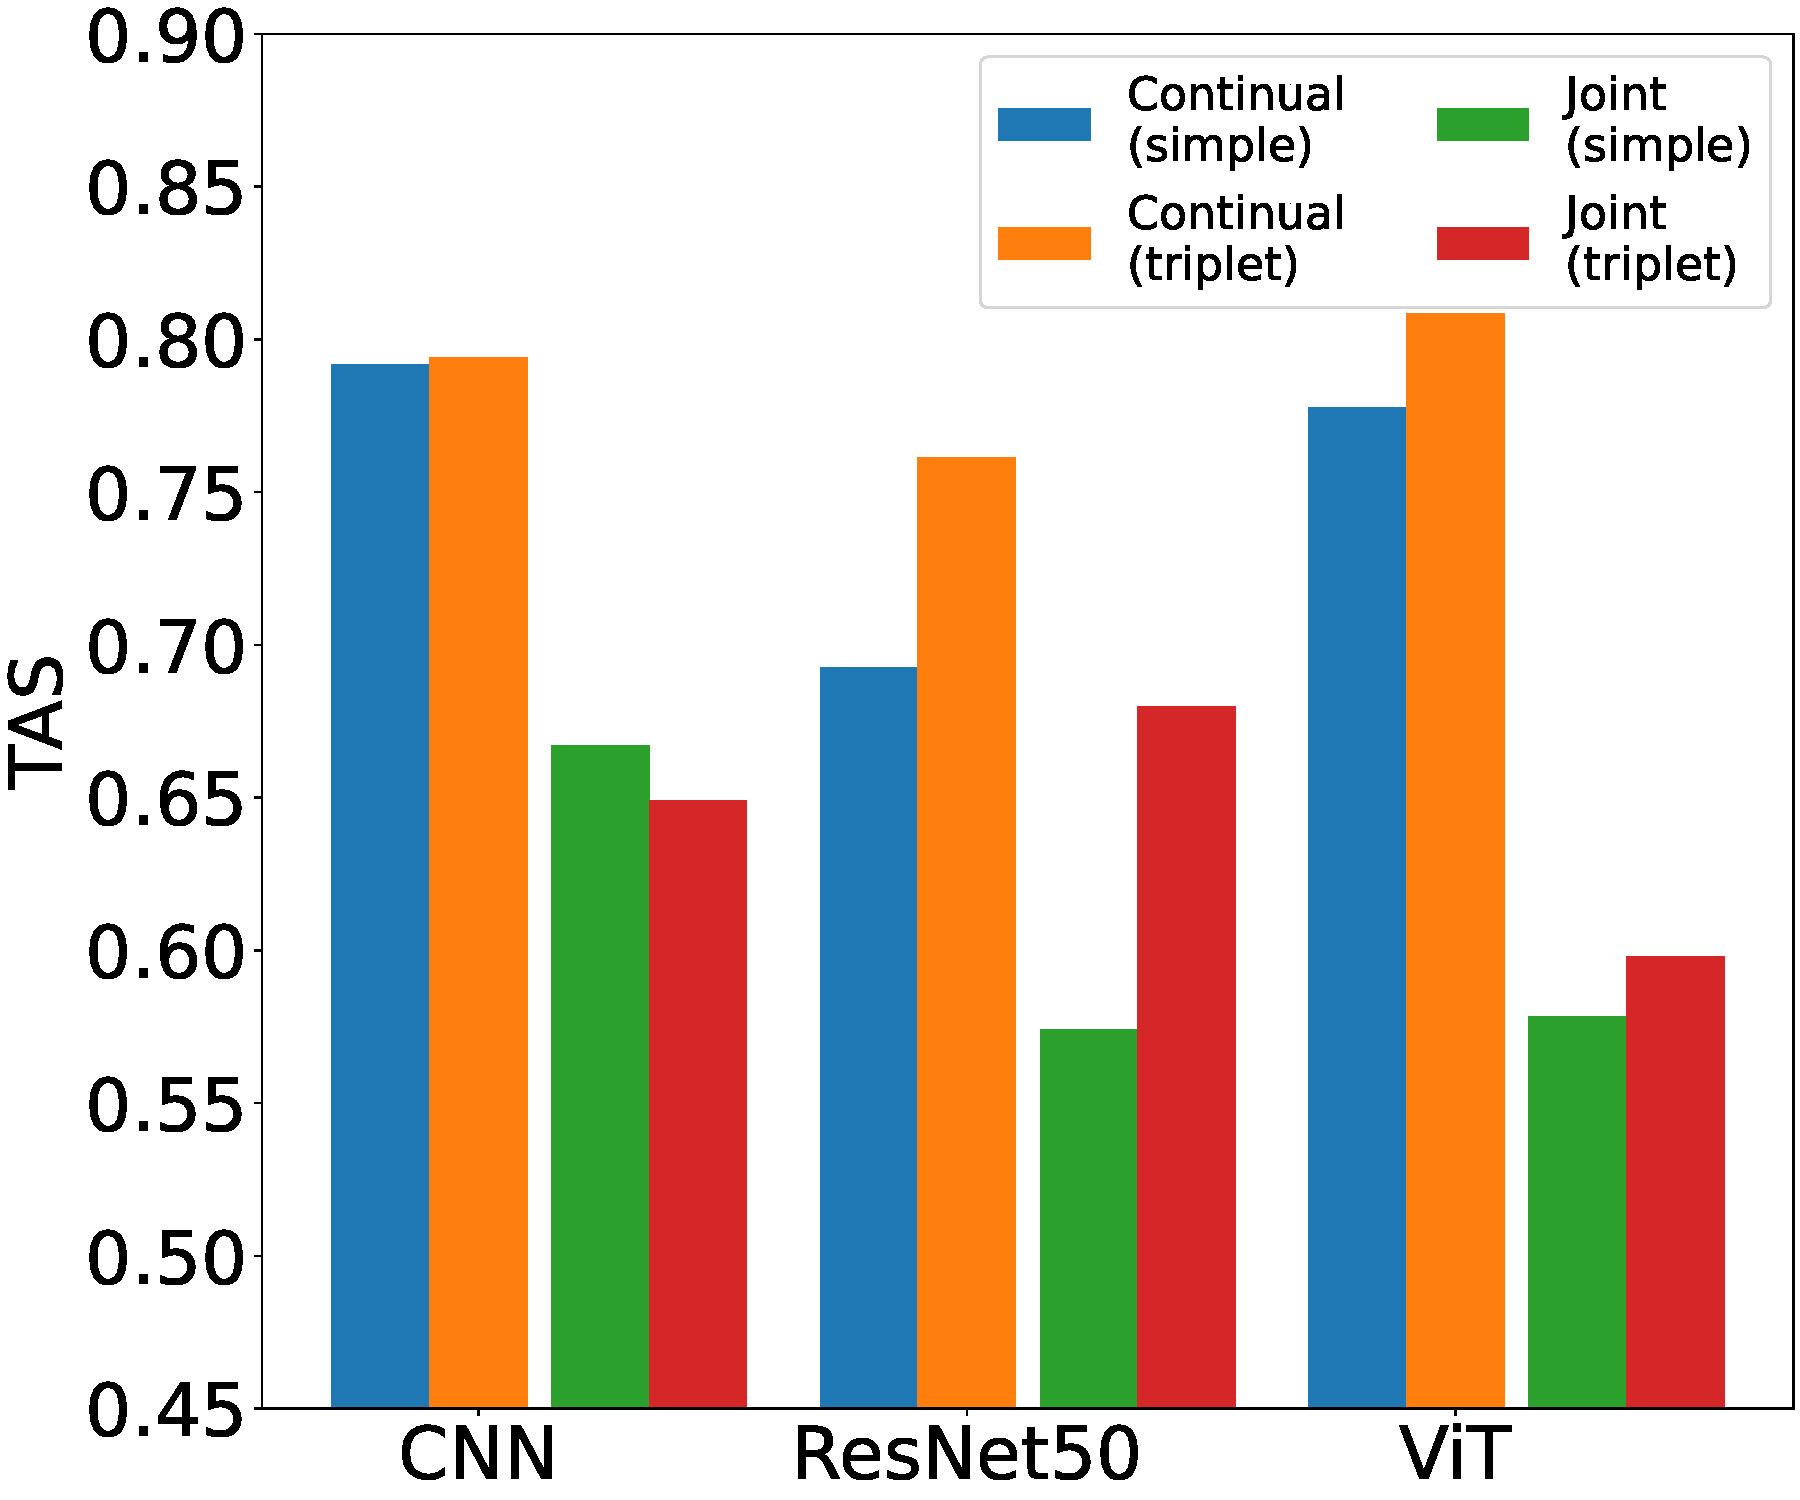
\includegraphics[width=\textwidth]{imgs/cem/KANDY_1-TAS_ablation.pdf}
	\caption{\textsc{KANDY-Concepts-1}}
	\end{subfigure}
	\begin{subfigure}{.49\textwidth}
		\centering
	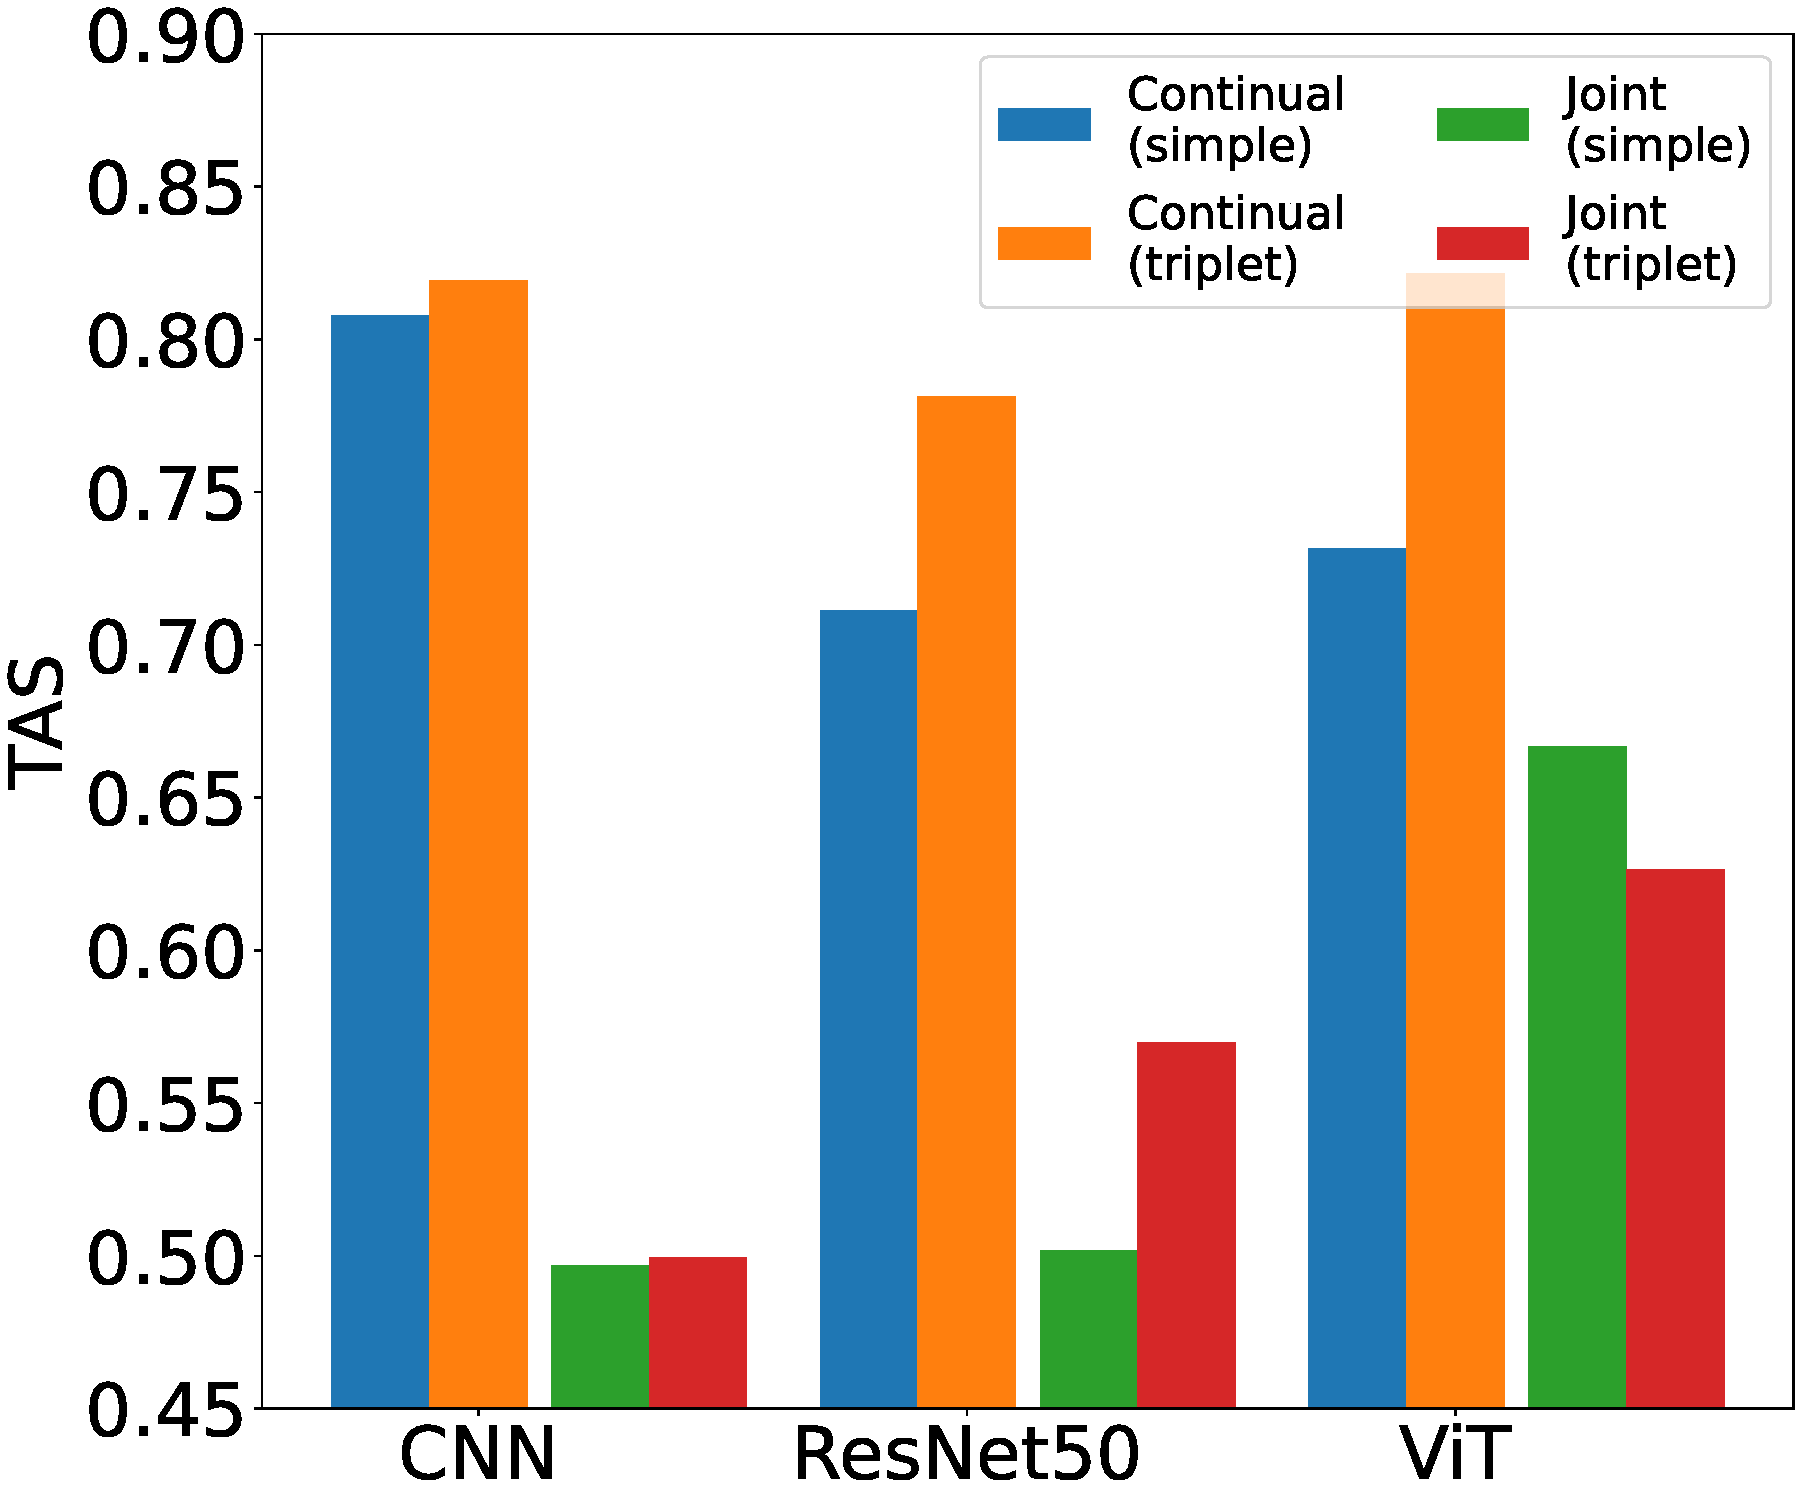
\includegraphics[width=\textwidth]{imgs/cem/KANDY_2-TAS_ablation.pdf}
	\caption{\textsc{KANDY-Concepts-2}}
	\end{subfigure}
	\caption[Concept alignment on \textsc{KANDY-Concepts}]{%The impact of the triplet loss in the learned concepts. For each model, we report the {\small\sc TAS} score without exploiting the proposed concept-level triplet loss (first bar of each pair - labeled ``simple'') and when using it (second bar - labeled ``triplet'').
		Task-concept alignment, Task-incremental (``Continual'') and Joint settings. We compare cases without triplet loss (``simple'') and with triplet loss (``triplet'').
		%\vspace{-2mm}
	}
	\label{cem:fig:tas-ablation}
\end{figure}


\paragraph{The Role of Time.} Figure~\ref{cem:fig:kandytime} (a, b, e, f) inspects the same results of Table~\ref{cem:tab:main}, with the addition of {\small\sc Average Forgetting} (c, g) and {\small \sc DIAGS} (d, h), reporting their values at different time instants (tasks). In \textsc{KANDY-Concepts-1} (Figure~\ref{cem:fig:kandytime} top) accuracy slowly decreases with the number of tasks, although not in a critical way. The \textsc{CNN} model shows low accuracy in some initial tasks. Forgetting, which is not critically high in the deeper models, shows a bump in the early tasks for \textsc{CNN}. This confirms that the more limited effect of the triplet loss in this model is caused by storing sub-optimal concepts in the buffer. Overall, the controlled level of forgetting is mostly due to the task-level experience replay. Interestingly, {\small\sc TAS} is relatively low in the first task, and it quickly increases during the following few tasks. This means that the models are able to capture the key concepts that are needed to learn the task almost since the beginning, and these concepts are not subject to uncontrolled dynamics, but they stay stable, confirming the role of concept-level replay.
These comments, overall, hold also in the case of \textsc{KANDY-Concepts-2} (Figure~\ref{cem:fig:kandytime} bottom) with some important differences. Accuracy is higher in the first tasks, suggesting that they can more easily be solved with the selected models. Forgetting seems to increase visibly, but mostly due to the larger number of tasks. In this case, the \textsc{CNN} shows evident forgetting issues at a later stage with respect to \textsc{KANDY-Concepts-1}, which, however, still supports our explanations on the triplet loss impact. {\small\sc TAS} confirms that the first tasks are easier to solve, and developing task-related concepts turns out to be easier as well.
\begin{figure}
\centering
%    \vskip -10mm
%    \begin{subfigure}{\textwidth}

\includegraphics[width=0.7\textwidth]{imgs/cem/legend.pdf}\\
%    \end{subfigure}
\begin{subfigure}{.24\textwidth}
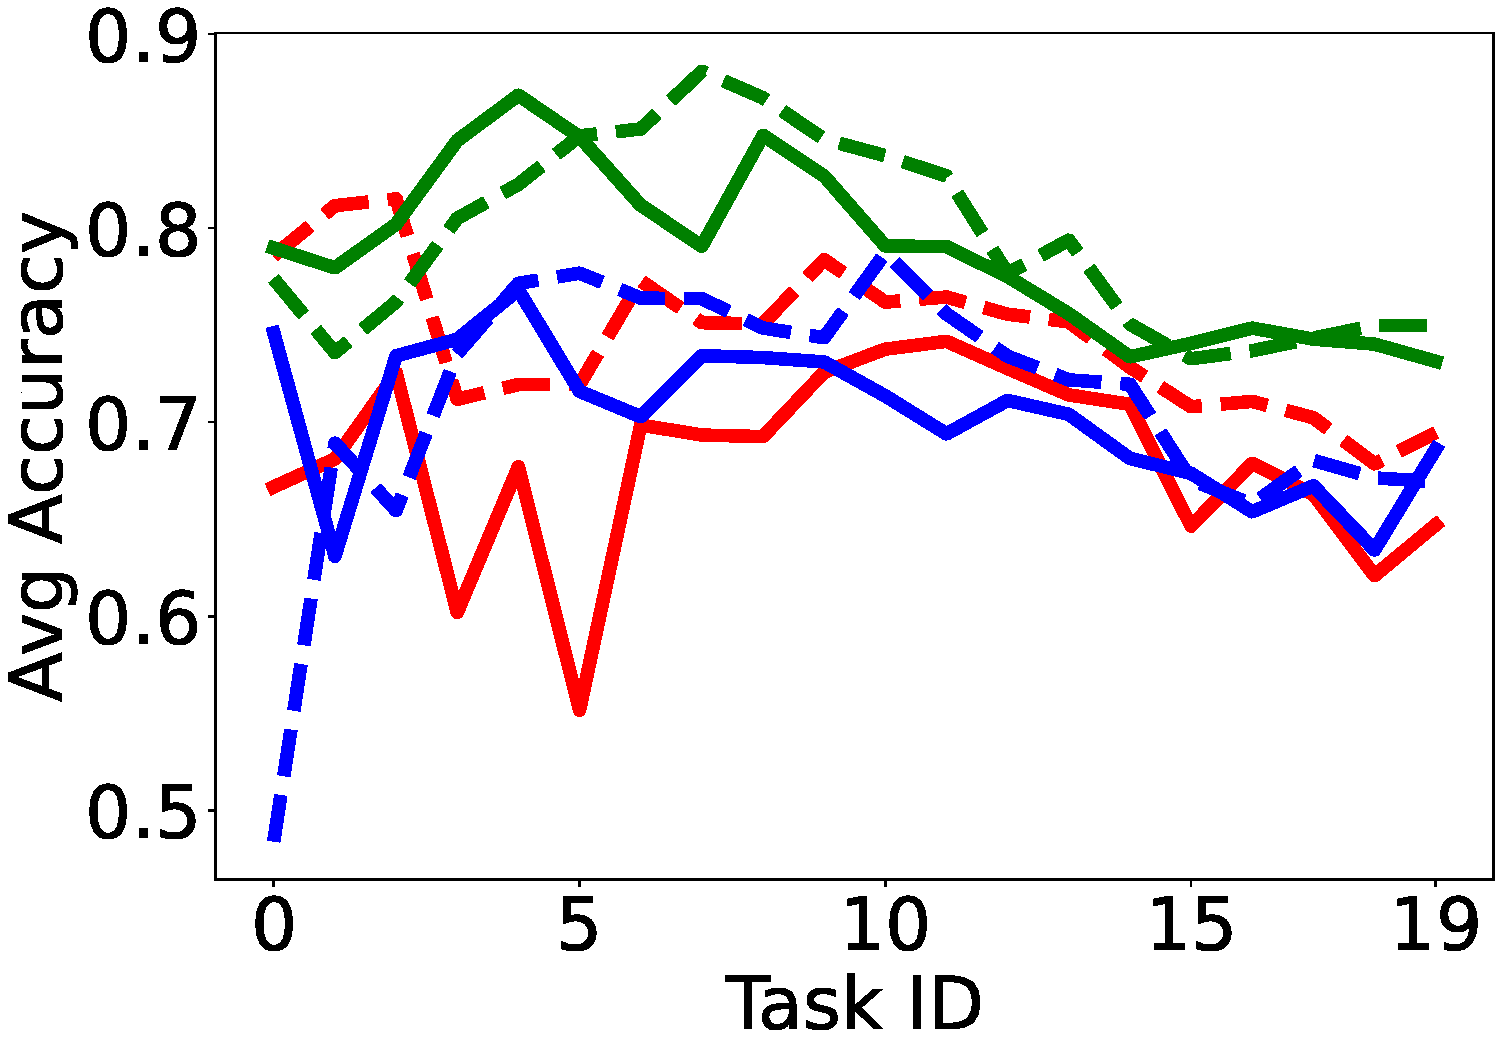
\includegraphics[width=\textwidth]{imgs/cem/KANDY_1_avg_accuracy-test.pdf}    
\caption{}
\end{subfigure}
\begin{subfigure}{.24\textwidth}
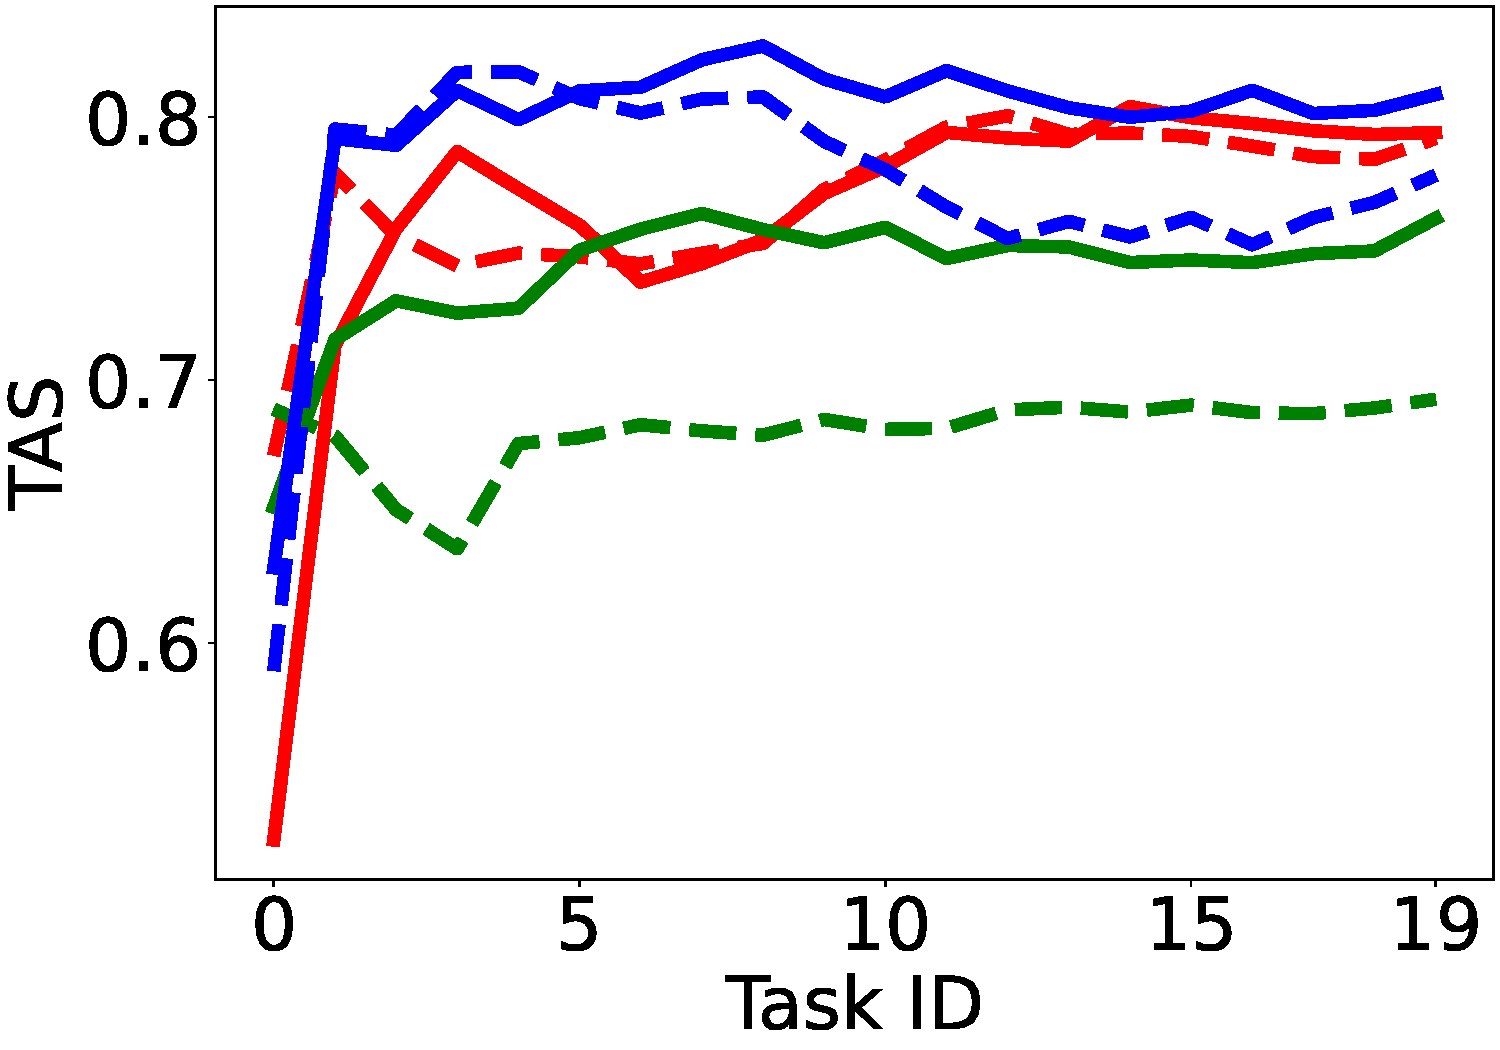
\includegraphics[width=\textwidth]{imgs/cem/KANDY_1_tas_extended-test.pdf}
\caption{}
\end{subfigure}    
\begin{subfigure}{.24\textwidth}
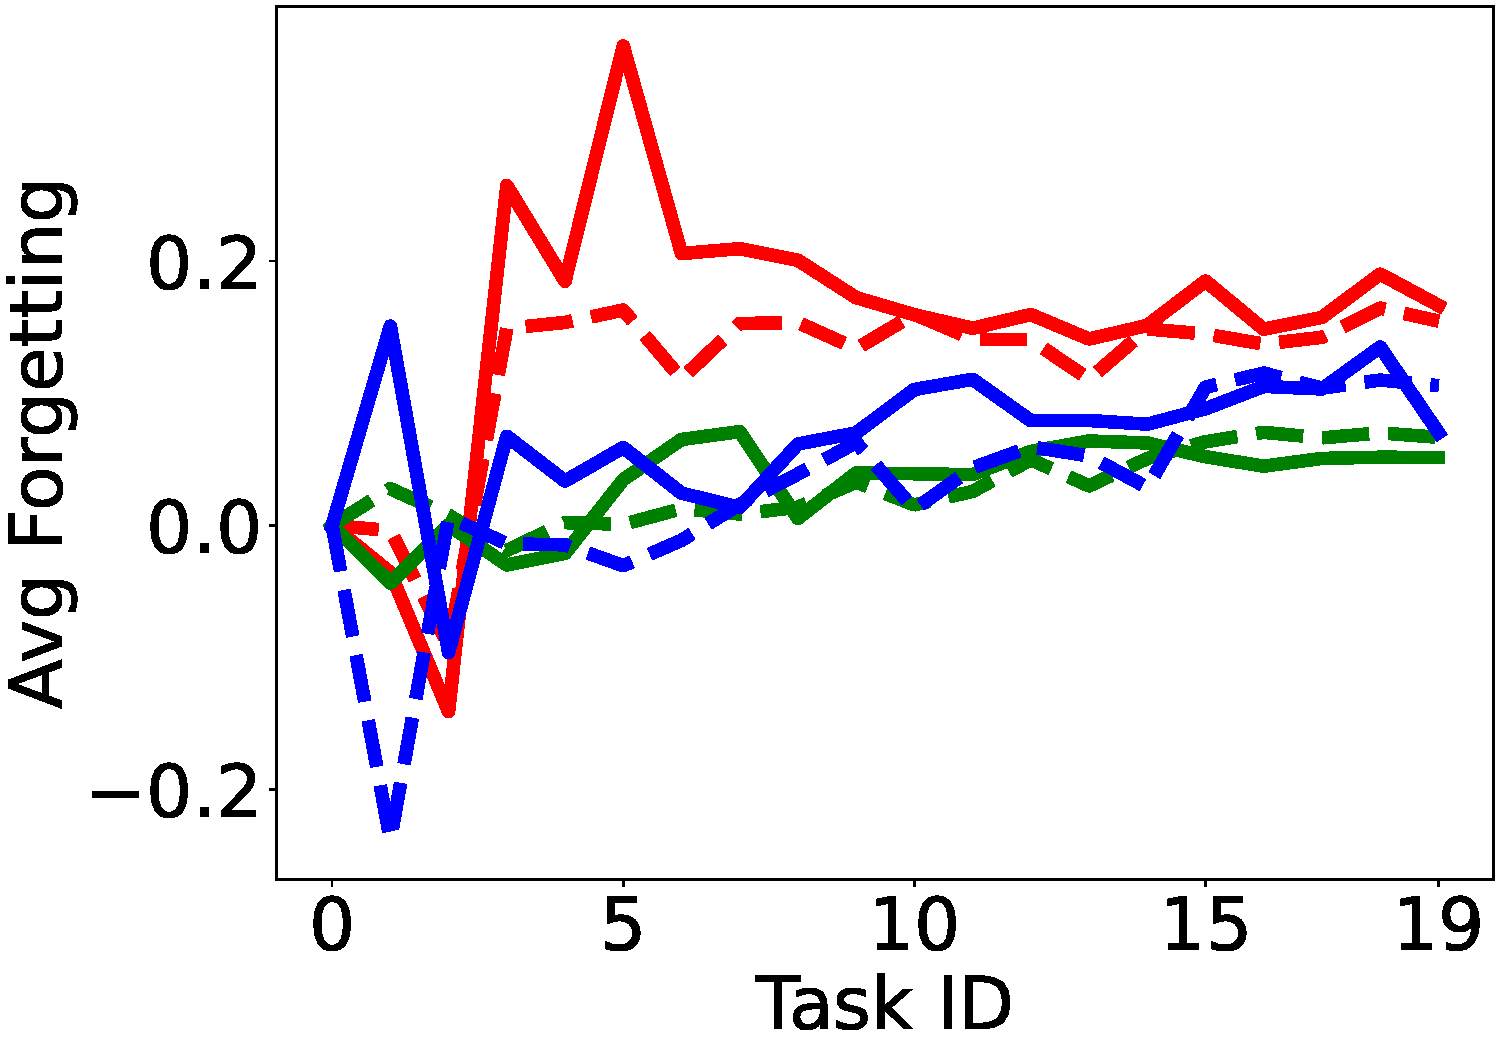
\includegraphics[width=\textwidth]{imgs/cem/KANDY_1_avg_forgetting-test.pdf}
\caption{}
\end{subfigure}
%\hfill
\begin{subfigure}{.24\textwidth}
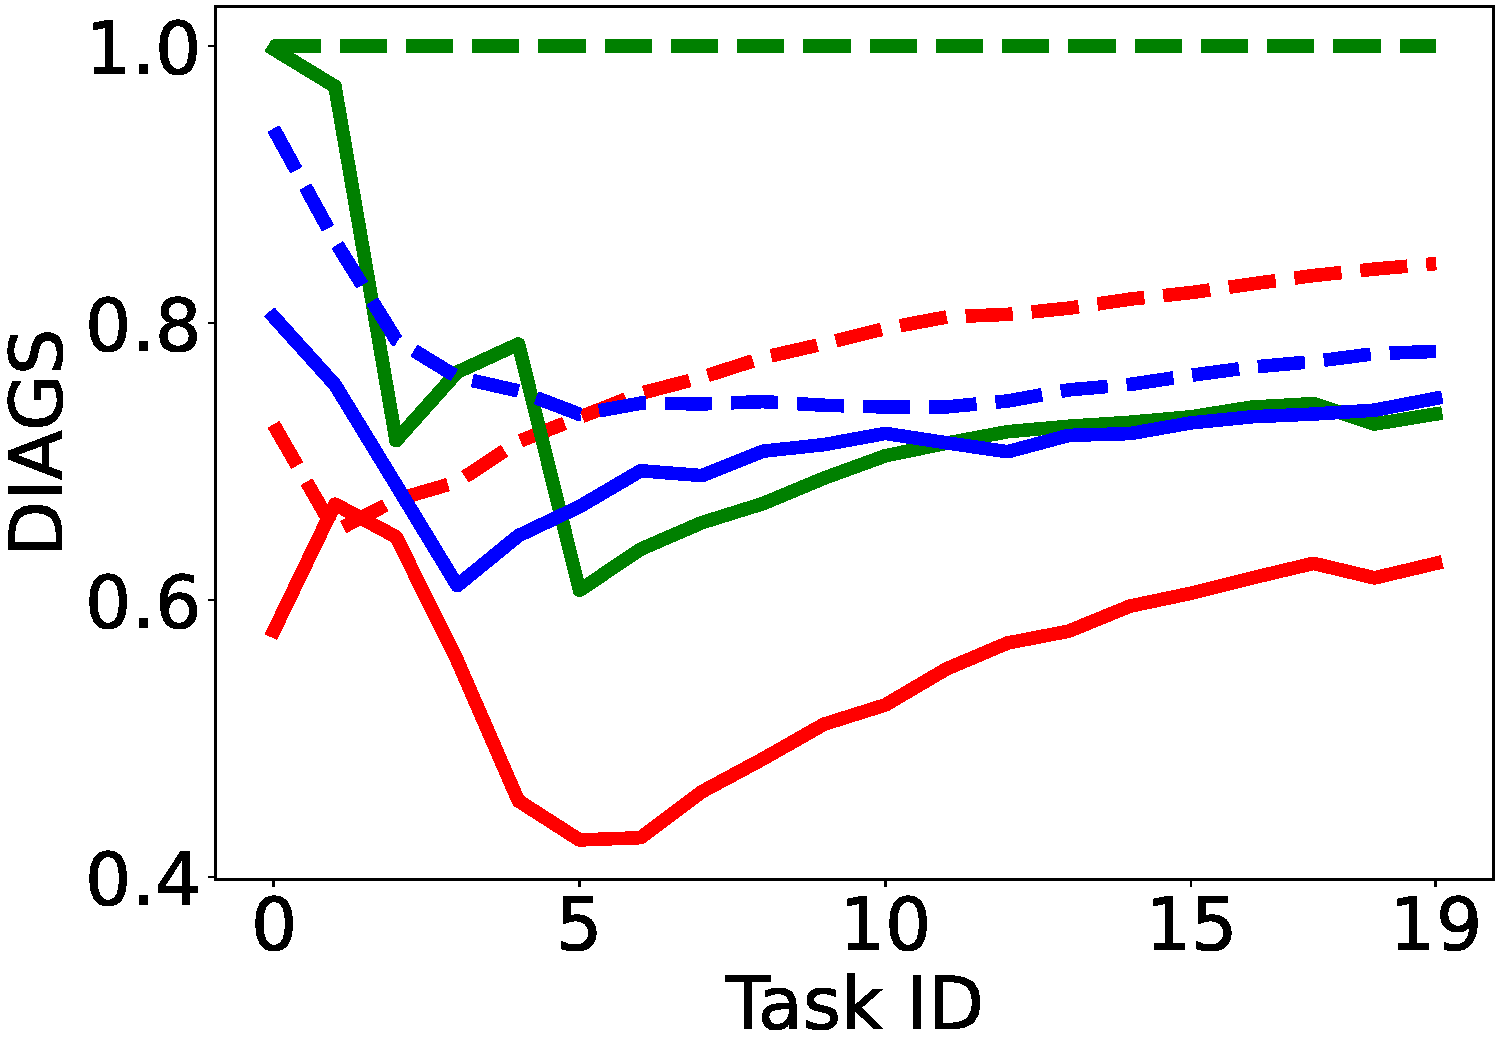
\includegraphics[width=\textwidth]{imgs/cem/KANDY_1_diagonalized_extended-test.pdf}   
\caption{}
\end{subfigure}
\begin{subfigure}{.24\textwidth}
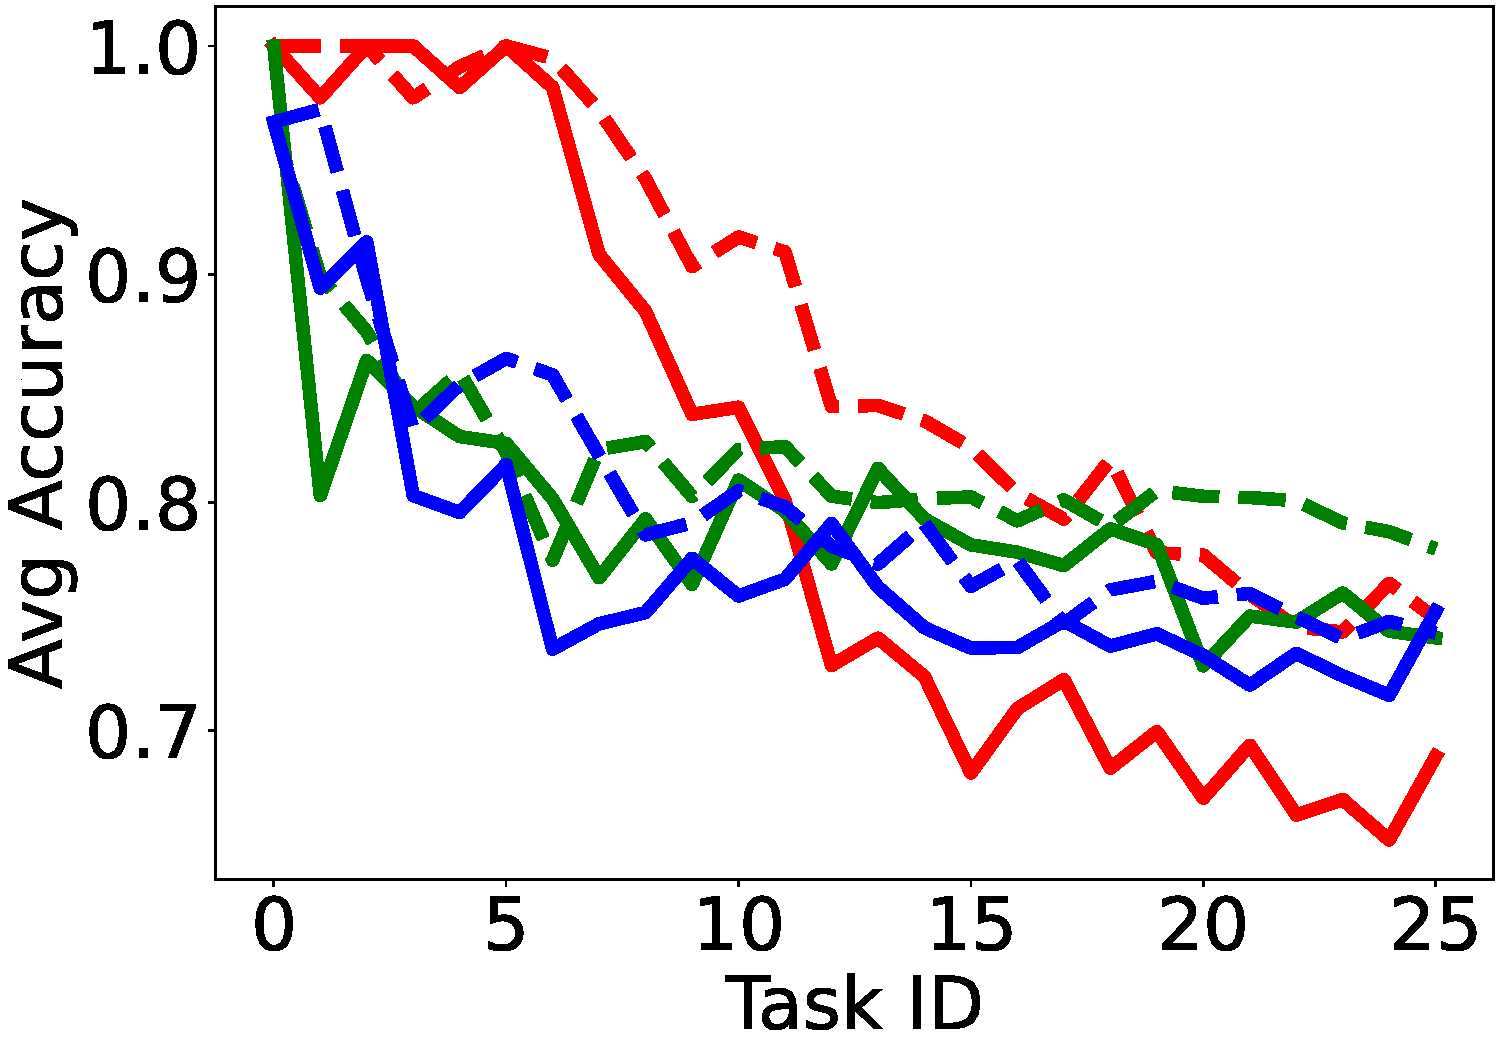
\includegraphics[width=\textwidth]{imgs/cem/KANDY_2_avg_accuracy-test.pdf}    
\caption{}
\end{subfigure}
\begin{subfigure}{.24\textwidth}
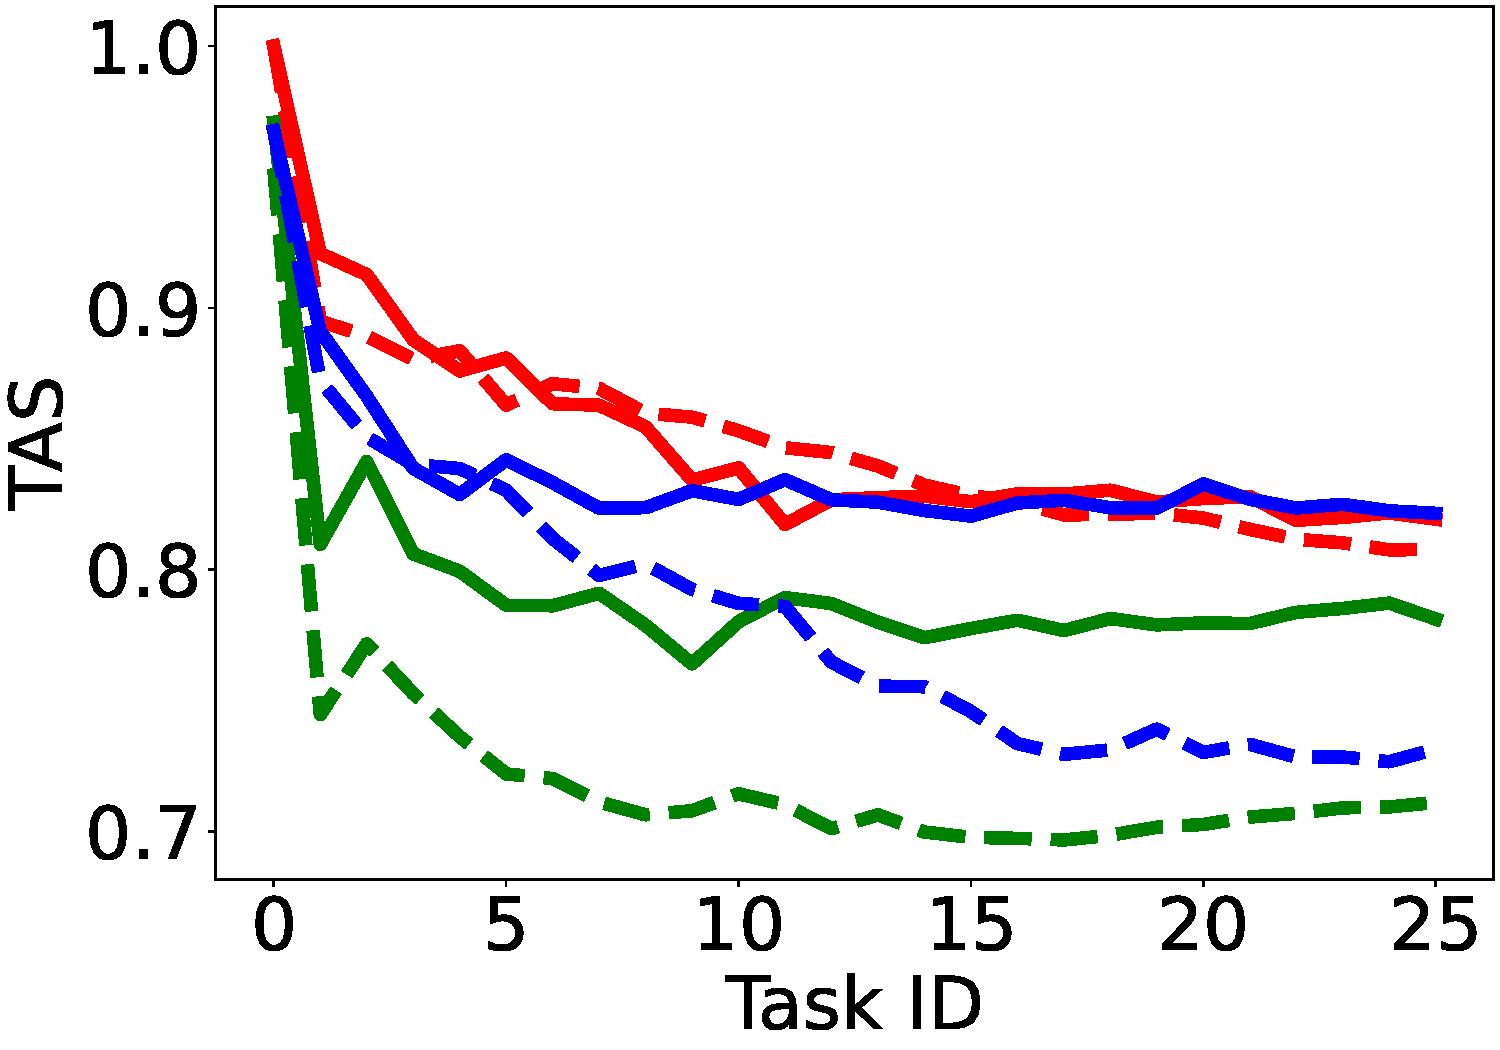
\includegraphics[width=\textwidth]{imgs/cem/KANDY_2_tas_extended-test.pdf}
\caption{}
\end{subfigure}     
%\hfill
\begin{subfigure}{.24\textwidth}
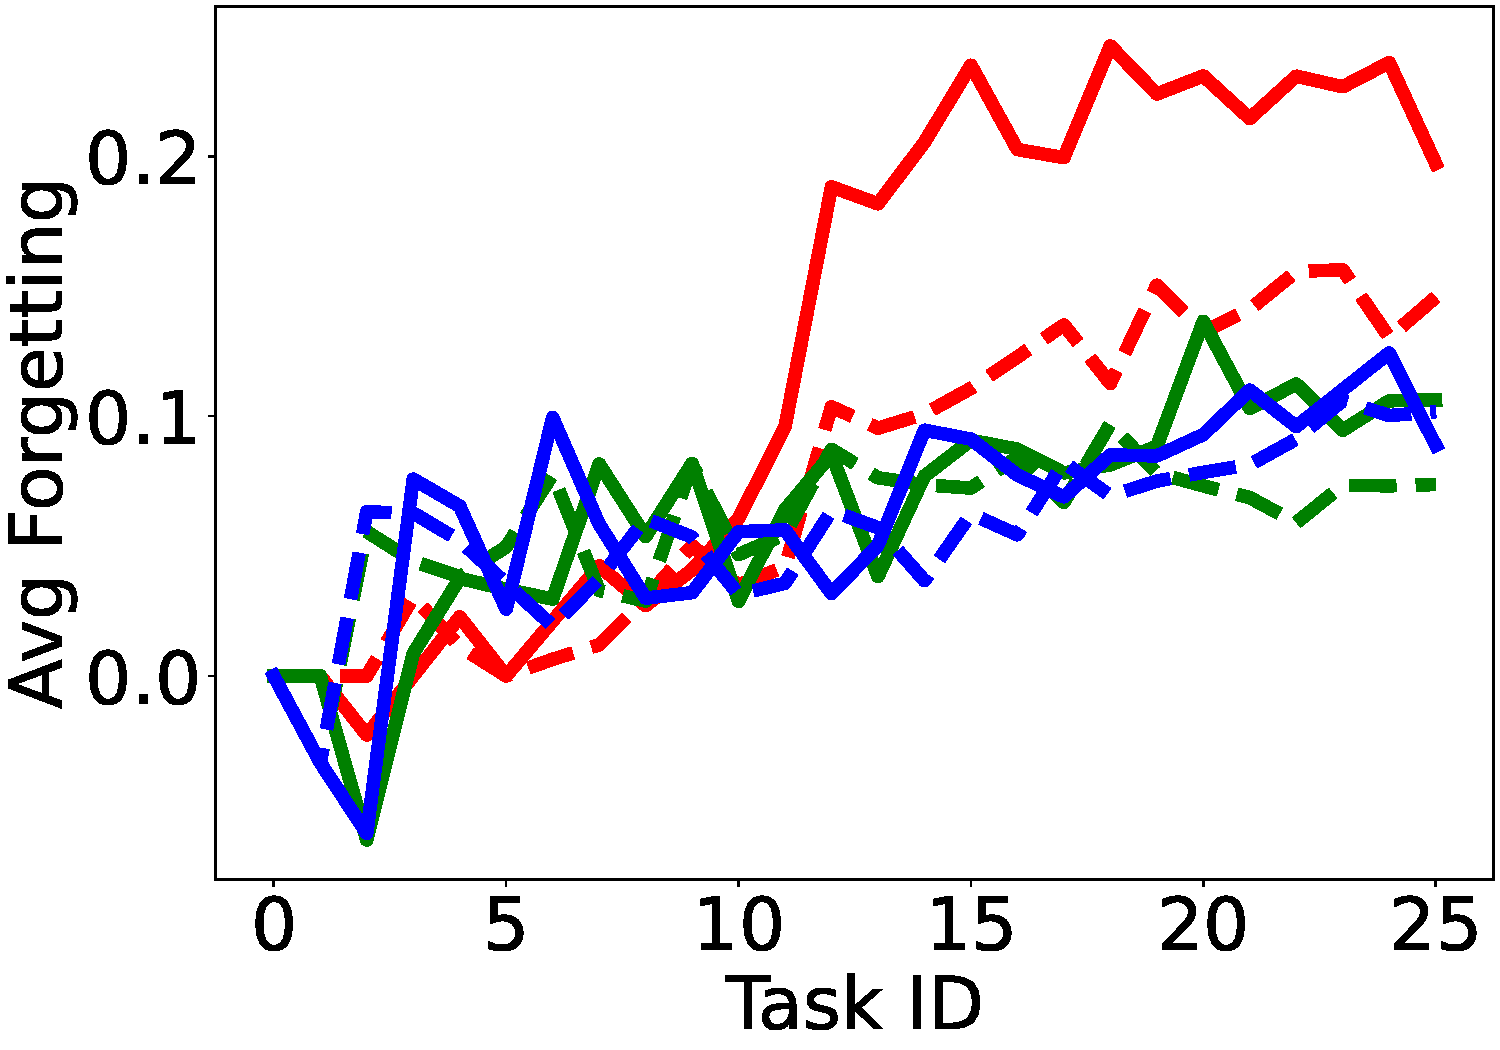
\includegraphics[width=\textwidth]{imgs/cem/KANDY_2_avg_forgetting-test.pdf}
\caption{}
\end{subfigure}   
\begin{subfigure}{.24\textwidth}
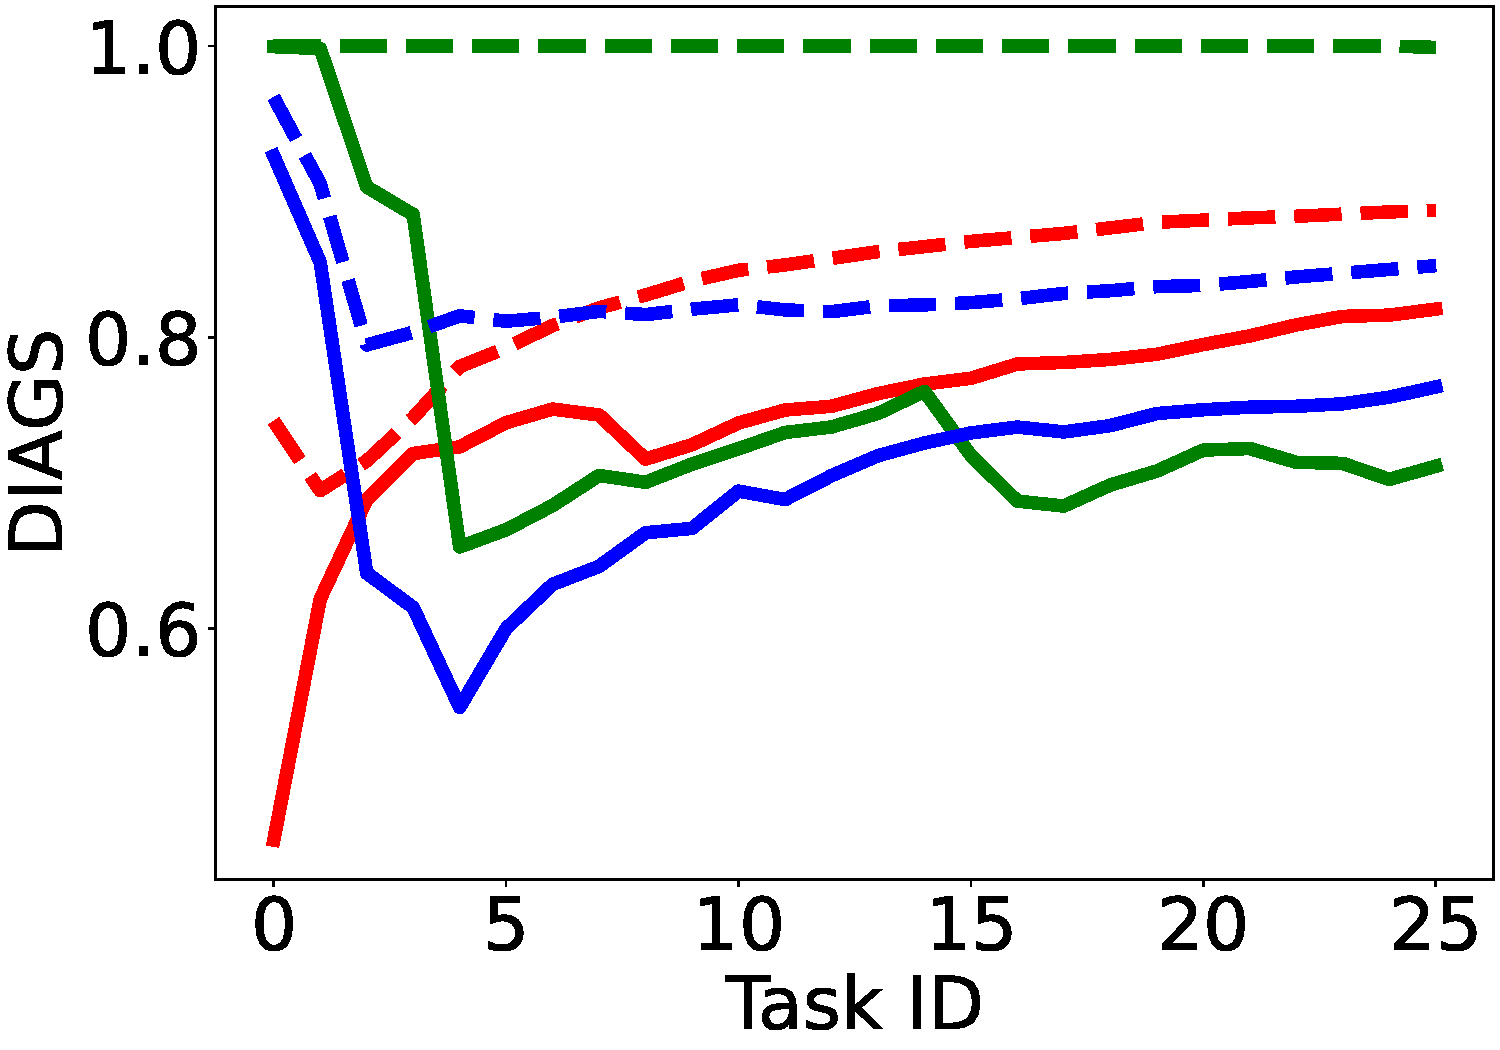
\includegraphics[width=\textwidth]{imgs/cem/KANDY_2_diagonalized_extended-test.pdf}   
\caption{}
\end{subfigure}
\caption[Performance over time on \textsc{KANDY-Concepts}]{Metrics evolution through time for \textsc{KANDY-Concepts-1} (top) and \textsc{KANDY-Concepts-2} (bottom): {\small\sc Average Accuracy} (a, e), {\small\sc TAS} (b, f), {\small\sc Average Forgetting} (c, g), {\small\sc Diags} (d, h). Solid (dashed) lines are with (without) triplet loss.
%\vspace{-4mm}
}
\label{cem:fig:kandytime}
\end{figure}

\paragraph{Concepts vs. Concepts.} Table~\ref{cem:tab:other-scores} reports more detailed results related to concept-level metrics. 
%We can observe how
In the Task-incremental setting, \textsc{KANDY-Concepts-2} yields more uncorrelated concepts (larger values of {\small\sc DIAGS}), which is desirable. When comparing the ground truth concepts with the learned ones ({\small\sc GCAS}, {\small\sc JSD-P}, {\small\sc JSD-T}), on average, the Task-incremental case is better suited to model our expectation (consistently smaller {\small\sc JSD-P}, mixed results for {\small\sc JSD-T} and {\small\sc GCAS}). However, when considering \textsc{KANDY-Concepts-1} we observe a different behavior. Joint training leads to better {\small\sc DIAGS}, although the already discussed lower {\small\sc TAS} (Table~\ref{cem:tab:main}) suggests that concepts, overall, are less related to the tasks with respect to the Task-incremental case, while being more uncorrelated. We motivate this result by the subpar accuracies in the first tasks of \textsc{KANDY-Concepts-1} (Task-incremental setting), which, paired with concept-level replay, leads to the development of some partially overlapping concepts over time. By comparing the ground truth concepts with the learned ones, we clearly see that the solution found in the Task-incremental case is less aligned with our expectations. The network is indeed finding solutions that are task-related (Table~\ref{cem:tab:main}), but not the ones we had hypothesized. 
%suggests that joint-training might leverage the concept embedding space of CEMs instead of directly using multiple concepts to solve the tasks. In fact, due to the unsupervised nature of the problem, CEMs are not forced to activate or not-activate concepts, since the values in $\vc$ are fully unconstrained.
%, typically better aligned with the ground-truth concepts (consistently smaller {\small\sc JSD-P}, mixed results for {\small\sc JSD-T} and {\small\sc GCAS}).
%
Overall, we argue that this difference between the two datasets is also likely due to the larger number of tasks and, more importantly, of ground truth concepts in \textsc{KANDY-Concepts-2}, where Joint training has to face the challenge of simultaneously discovering several concepts, which are instead disclosed gradually in the Task-incremental setting. %In general, the relationships between concept discovery and dataset characteristics seem to play an interesting role which will be subject to further investigation.%be very interesting and will certainly be the subject of further investigations.

\paragraph{Correlation Matrices.} We investigate more detailed results characterizing concept-level metrics, reporting a visual example about the Matthews Correlation Coefficient, in Figure~\ref{cem:fig:mcc} (\textsc{KANDY-Concepts-2}, \textsc{ViT-16}). In Figure~\ref{cem:fig:mcc} (a, b), we show the correlation among the automatically discovered concepts. In (a) the triplet loss is not used, while in (b) it is active. In the latter case, we clearly see the filled diagonal, while in the former there is an unused concept, suggesting that the triplet loss favors the usage of the available resources. However, when the triplet loss is used, we also see some more positive correlations (more reddish, orange areas), suggesting that there is indeed a bit more overlap among concepts. In Figure~\ref{cem:fig:mcc} (c, d) we report the correlation matrix between the learned concepts (rows) and the ground truth ones (columns), without (c) and with triplet loss (d). In the latter case it is easy to see that there are some dark horizontal stripes that are missing in (c). This suggests that some learned concepts (the ones of the darker rows) are either not used much or that they encode properties far from the ground truth. This behavior is expected, since there is nothing preventing the network from encoding additional information with respect to our expectations. In the Joint learning case, due to the immediate availability of the data from all tasks, the ground truth concepts are more spread across the learned ones.

\begin{table}
\centering
\resizebox{\textwidth}{!}{\begin{tabular}{cccccccccc}
\toprule
\multirow{2}{*}{\sc Model} & \multirow{2}{*}{\sc Setting} & \multicolumn{4}{c}{{\small\sc KANDY-Concepts-1}} & \multicolumn{4}{c}{{\small\sc KANDY-Concepts-2}} \\
\cmidrule{3-10}
& & {\small\sc \underline{DIAGS}} $\uparrow$ & {\small\sc GCAS} $\uparrow$ & {\small\sc JSD-T} $\downarrow$ & {\small\sc JSD-P} $\downarrow$  & {\small\sc \underline{DIAGS}} $\uparrow$ & {\small\sc GCAS} $\uparrow$ & {\small\sc JSD-T} $\downarrow$ & {\small\sc JSD-P} $\downarrow$ \\
\midrule
\multirow{2}{*}{CNN} &
%Continual & 0.63 $$ {\tiny ($\pm 0.02$)} & 0.58 $$ {\tiny ($\pm 0.01$)} & 13.81 $$ {\tiny ($\pm 0.57$)} & 2.90 $$ {\tiny ($\pm 0.07$)} & \cellcolor{Gray}\textbf{0.82} $$ {\tiny ($\pm 0.03$)} & \cellcolor{Gray}0.60 $$ {\tiny ($\pm 0.00$)} & \cellcolor{Gray}11.06 $$ {\tiny ($\pm 0.85$)} & \cellcolor{Gray}\textbf{4.53} $$ {\tiny ($\pm 0.28$)} \\
Task-incremental & 0.63 $$ {\tiny ($\pm 0.02$)} & 0.58 $$ {\tiny ($\pm 0.01$)} & 13.81 $$ {\tiny ($\pm 0.57$)} & 2.90 $$ {\tiny ($\pm 0.07$)} & \textbf{0.82} $$ {\tiny ($\pm 0.03$)} & 0.60 $$ {\tiny ($\pm 0.00$)} & 11.06 $$ {\tiny ($\pm 0.85$)} & \textbf{4.53} $$ {\tiny ($\pm 0.28$)} \\
%& Joint & \cellcolor{Gray}{\bf 0.96 $$ {\tiny ($\pm 0.03$)}} & \cellcolor{Gray}\textbf{0.66 $$ {\tiny ($\pm 0.01$)}} & \cellcolor{Gray}\textbf{6.53} $$ {\tiny ($\pm 2.04$)} & \cellcolor{Gray}\textbf{1.88} $$ {\tiny ($\pm 0.42$)} & 0.52 $$ {\tiny ($\pm 0.07$)} & \textbf{0.65} $$ {\tiny ($\pm 0.02$)} & {\bf 10.02 $$ {\tiny ($\pm 0.30$)}} & 4.91 $$ {\tiny ($\pm 0.07$)} \vspace{-1mm}\\
& Joint & {\bf 0.96 $$ {\tiny ($\pm 0.03$)}} & \textbf{0.66 $$ {\tiny ($\pm 0.01$)}} & \textbf{6.53} $$ {\tiny ($\pm 2.04$)} & \textbf{1.88} $$ {\tiny ($\pm 0.42$)} & 0.52 $$ {\tiny ($\pm 0.07$)} & \textbf{0.65} $$ {\tiny ($\pm 0.02$)} & {\bf 10.02 $$ {\tiny ($\pm 0.30$)}} & 4.91 $$ {\tiny ($\pm 0.07$)} \\
\hdashline
\multirow{2}{*}{ResNet-50} &
%Continual & 0.73 $$ {\tiny ($\pm 0.02$)} & 0.62 $$ {\tiny ($\pm 0.00$)} & 14.05 $$ {\tiny ($\pm 0.86$)} & 2.97 $$ {\tiny ($\pm 0.07$)} & \cellcolor{Gray}{\bf 0.71 $$ {\tiny ($\pm 0.03$)}} & \cellcolor{Gray}0.58 $$ {\tiny ($\pm 0.00$)} & \cellcolor{Gray}{\bf 10.75 $$ {\tiny ($\pm 1.34$)}} & \cellcolor{Gray}{\bf 4.58 $$ {\tiny ($\pm 0.18$)}} \\
Task-incremental & 0.73 $$ {\tiny ($\pm 0.02$)} & 0.62 $$ {\tiny ($\pm 0.00$)} & 14.05 $$ {\tiny ($\pm 0.86$)} & 2.97 $$ {\tiny ($\pm 0.07$)} & {\bf 0.71 $$ {\tiny ($\pm 0.03$)}} & 0.58 $$ {\tiny ($\pm 0.00$)} & {\bf 10.75 $$ {\tiny ($\pm 1.34$)}} & {\bf 4.58 $$ {\tiny ($\pm 0.18$)}} \\
%& Joint & \cellcolor{Gray}\textbf{0.89} $$ {\tiny ($\pm 0.02$)} & \cellcolor{Gray}{\bf 0.70 $$ {\tiny ($\pm 0.01$)}} & \cellcolor{Gray}{\bf 10.73 $$ {\tiny ($\pm 1.03$)}} & \cellcolor{Gray}\textbf{1.88} $$ {\tiny ($\pm 0.10$)} & 0.58 $$ {\tiny ($\pm 0.04$)} & {\bf 0.62 $$ {\tiny ($\pm 0.02$)}} & 10.82 $$ {\tiny ($\pm 0.57$)} & 4.67 $$ {\tiny ($\pm 0.22$)} \vspace{-1mm}\\
& Joint & \textbf{0.89} $$ {\tiny ($\pm 0.02$)} & {\bf 0.70 $$ {\tiny ($\pm 0.01$)}} & {\bf 10.73 $$ {\tiny ($\pm 1.03$)}} & \textbf{1.88} $$ {\tiny ($\pm 0.10$)} & 0.58 $$ {\tiny ($\pm 0.04$)} & {\bf 0.62 $$ {\tiny ($\pm 0.02$)}} & 10.82 $$ {\tiny ($\pm 0.57$)} & 4.67 $$ {\tiny ($\pm 0.22$)} \\
\hdashline
\multirow{2}{*}{ViT-16} &
%Continual & 0.75 $$ {\tiny ($\pm 0.05$)} & 0.60 $$ {\tiny ($\pm 0.00$)} & 13.54 $$ {\tiny ($\pm 0.31$)} & 3.06 $$ {\tiny ($\pm 0.03$)} & \cellcolor{Gray}{\bf 0.77 $$ {\tiny ($\pm 0.03$)}} & \cellcolor{Gray}{\bf 0.58 $$ {\tiny ($\pm 0.00$)}} & \cellcolor{Gray}11.05 $$ {\tiny ($\pm 0.37$)} & \cellcolor{Gray}{\bf 4.58 $$ {\tiny ($\pm 0.10$)}} \\
Task-incremental & 0.75 $$ {\tiny ($\pm 0.05$)} & 0.60 $$ {\tiny ($\pm 0.00$)} & 13.54 $$ {\tiny ($\pm 0.31$)} & 3.06 $$ {\tiny ($\pm 0.03$)} & {\bf 0.77 $$ {\tiny ($\pm 0.03$)}} & {\bf 0.58 $$ {\tiny ($\pm 0.00$)}} & 11.05 $$ {\tiny ($\pm 0.37$)} & {\bf 4.58 $$ {\tiny ($\pm 0.10$)}} \\
%& Joint & \cellcolor{Gray}\textbf{0.85} $$ {\tiny ($\pm 0.03$)} & \cellcolor{Gray}{\bf 0.70 $$ {\tiny ($\pm 0.00$)}} & \cellcolor{Gray}{\bf 12.20 $$ {\tiny ($\pm 1.54$)}} & \cellcolor{Gray}{\bf 2.17 $$ {\tiny ($\pm 0.07$)}} & 0.55 $$ {\tiny ($\pm 0.10$)} & 0.56 $$ {\tiny ($\pm 0.01$)} & \textbf{9.79} $$ {\tiny ($\pm 1.35$)} & 4.73 $$ {\tiny ($\pm 0.20$)}\\
& Joint & \textbf{0.85} $$ {\tiny ($\pm 0.03$)} & {\bf 0.70 $$ {\tiny ($\pm 0.00$)}} & {\bf 12.20 $$ {\tiny ($\pm 1.54$)}} & {\bf 2.17 $$ {\tiny ($\pm 0.07$)}} & 0.55 $$ {\tiny ($\pm 0.10$)} & 0.56 $$ {\tiny ($\pm 0.01$)} & \textbf{9.79} $$ {\tiny ($\pm 1.35$)} & 4.73 $$ {\tiny ($\pm 0.20$)}\\
\bottomrule
\end{tabular}}
\caption[Concept alignment metrics for \textsc{KANDY-Concepts}]{Correlations between discovered concepts and (expected) ground truth concepts. Results are shown as $mean \pm std$ across 5 runs.}%, to remark cases in which the discovered concepts encode different information among them (larger {\small\sc DIAGS}), and there is a signal of improved correlation between discovered and expected concepts. In KANDY-2, due to the larger number of tasks and, more specifically, ground truth concept, the continual learning setting allows the network to find better solutions.%\vspace{-3mm}

\label{cem:tab:other-scores}
\end{table}

\begin{figure}
\centering
\begin{minipage}{.49\textwidth}
	\centering
	{\small\sc Discovered Concepts\\vs.\\Discovered Concepts}\\
	\begin{subfigure}{.49\textwidth}
		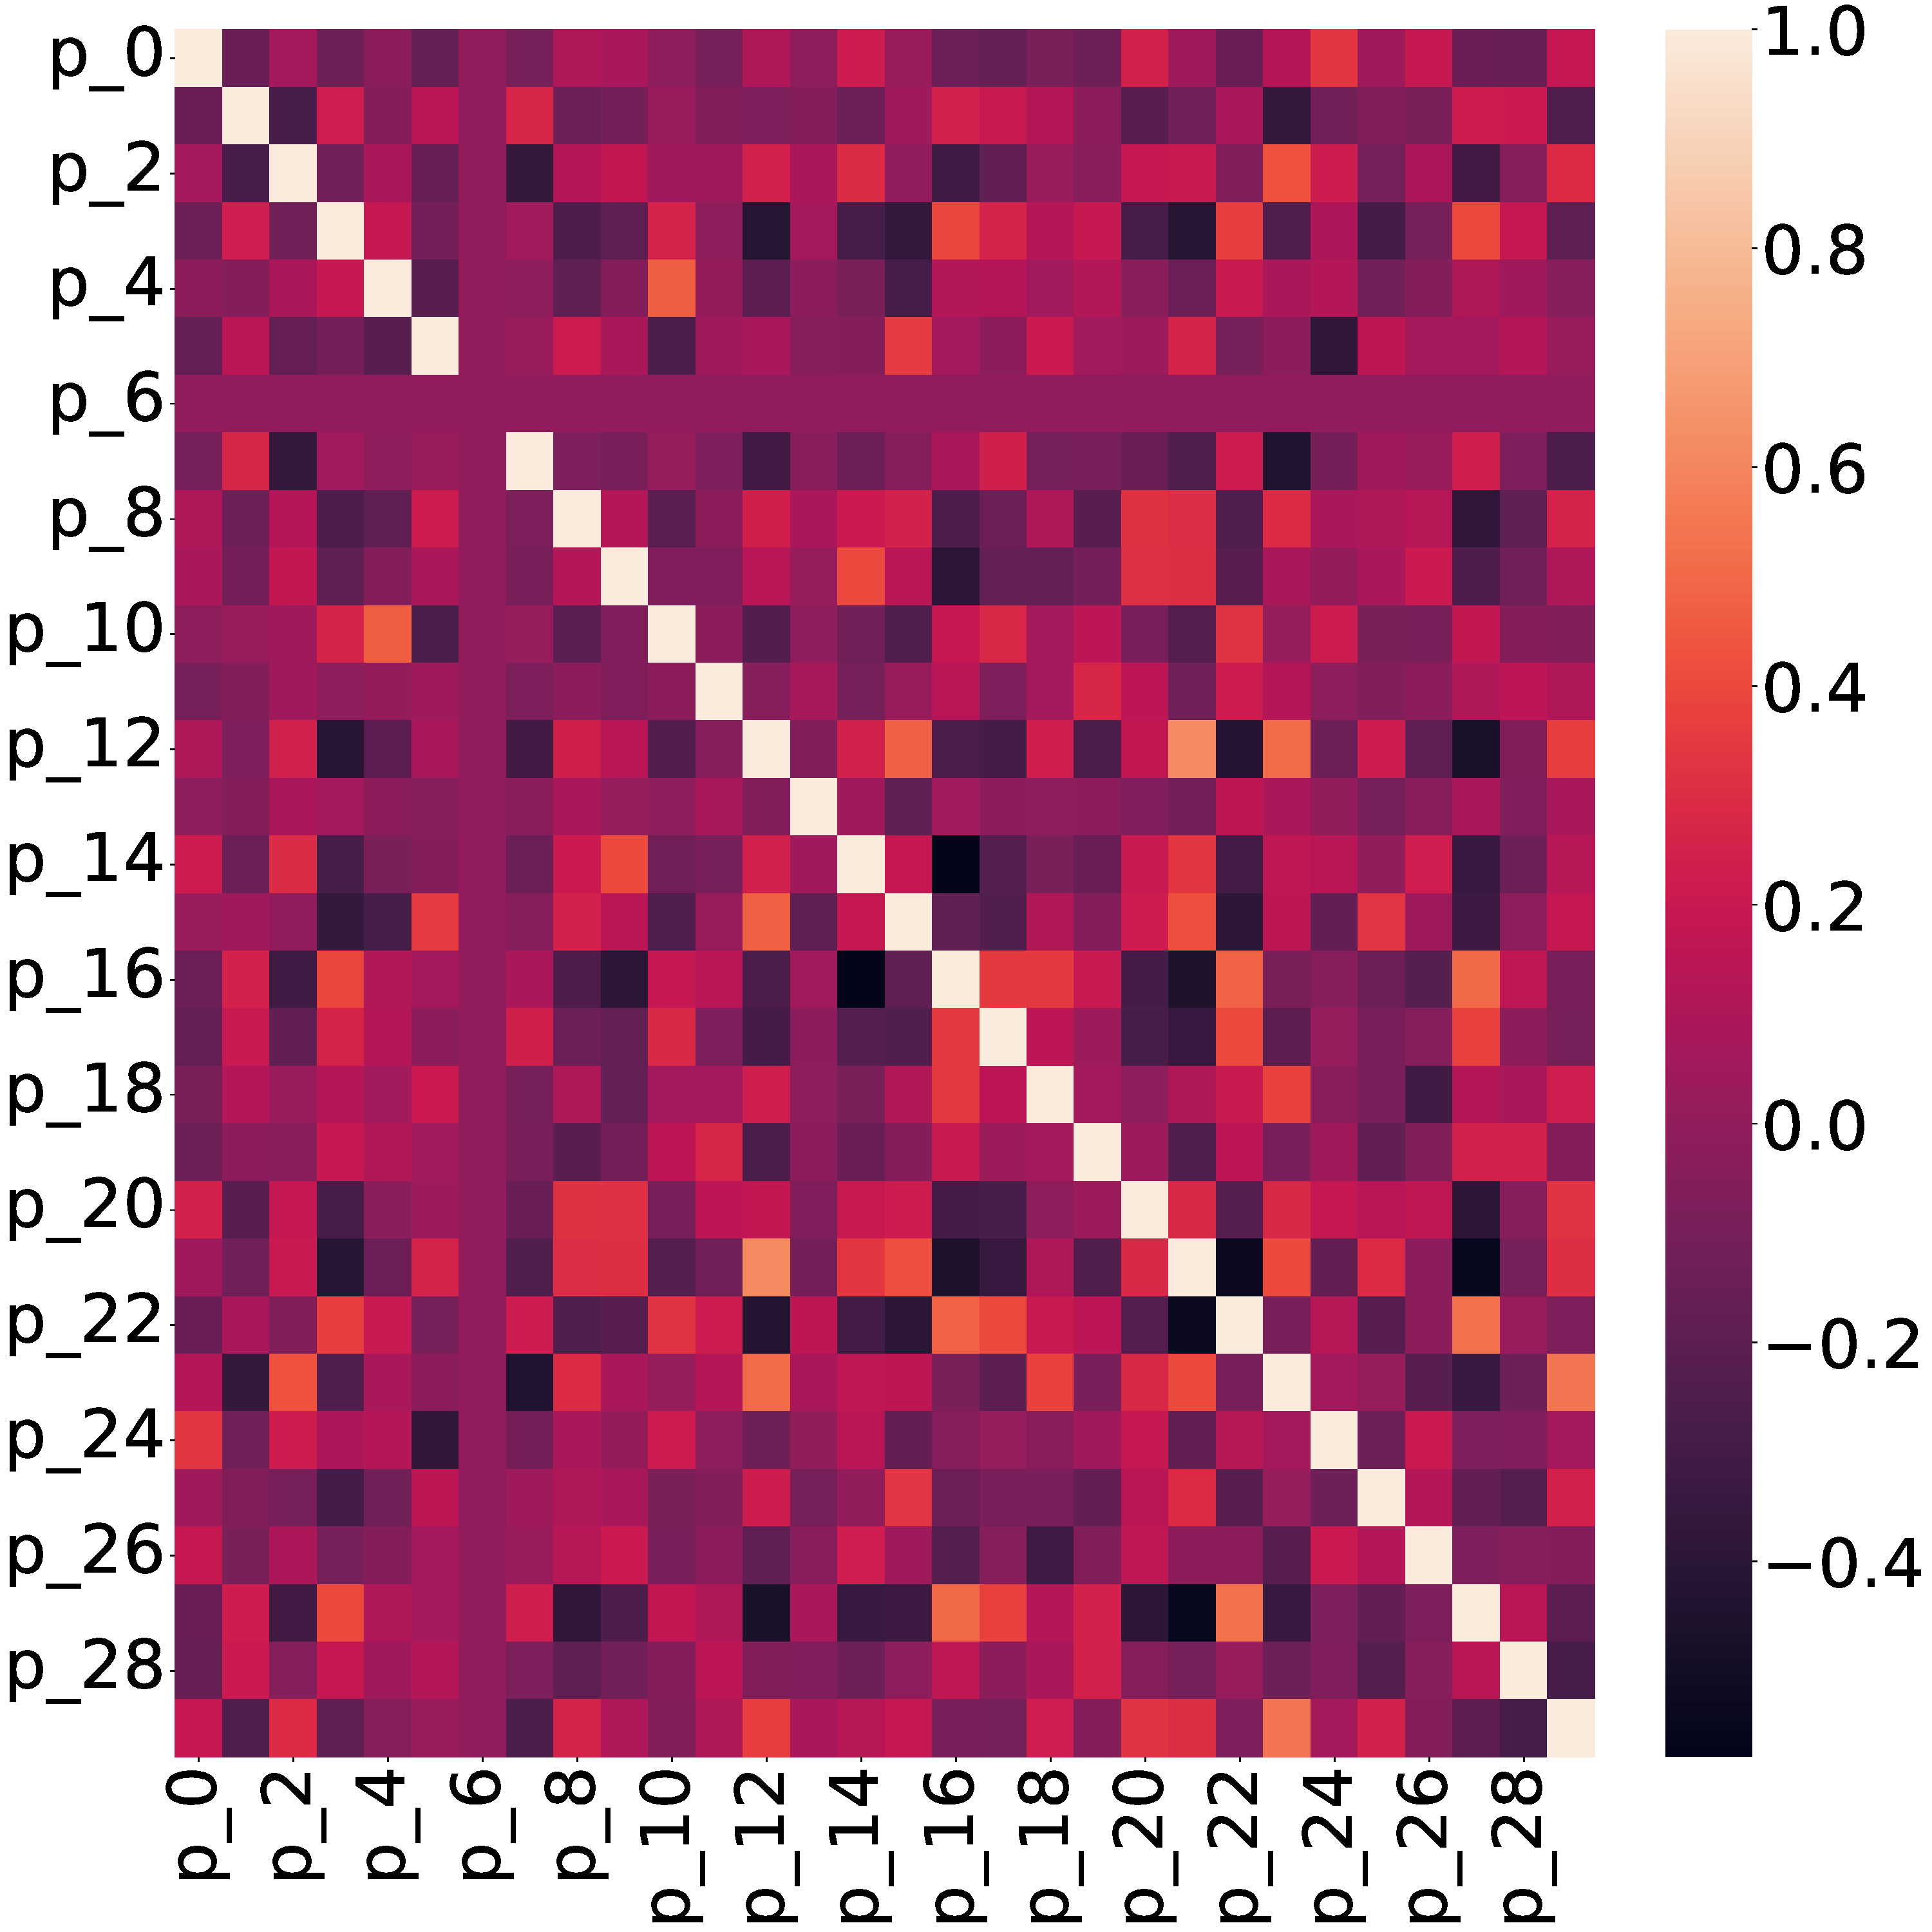
\includegraphics[width=\textwidth]{imgs/cem/KANDY_2-vit-continual-notriplet_pp.pdf}
		\caption{Simple}
	\end{subfigure}
	\begin{subfigure}{.49\textwidth}
		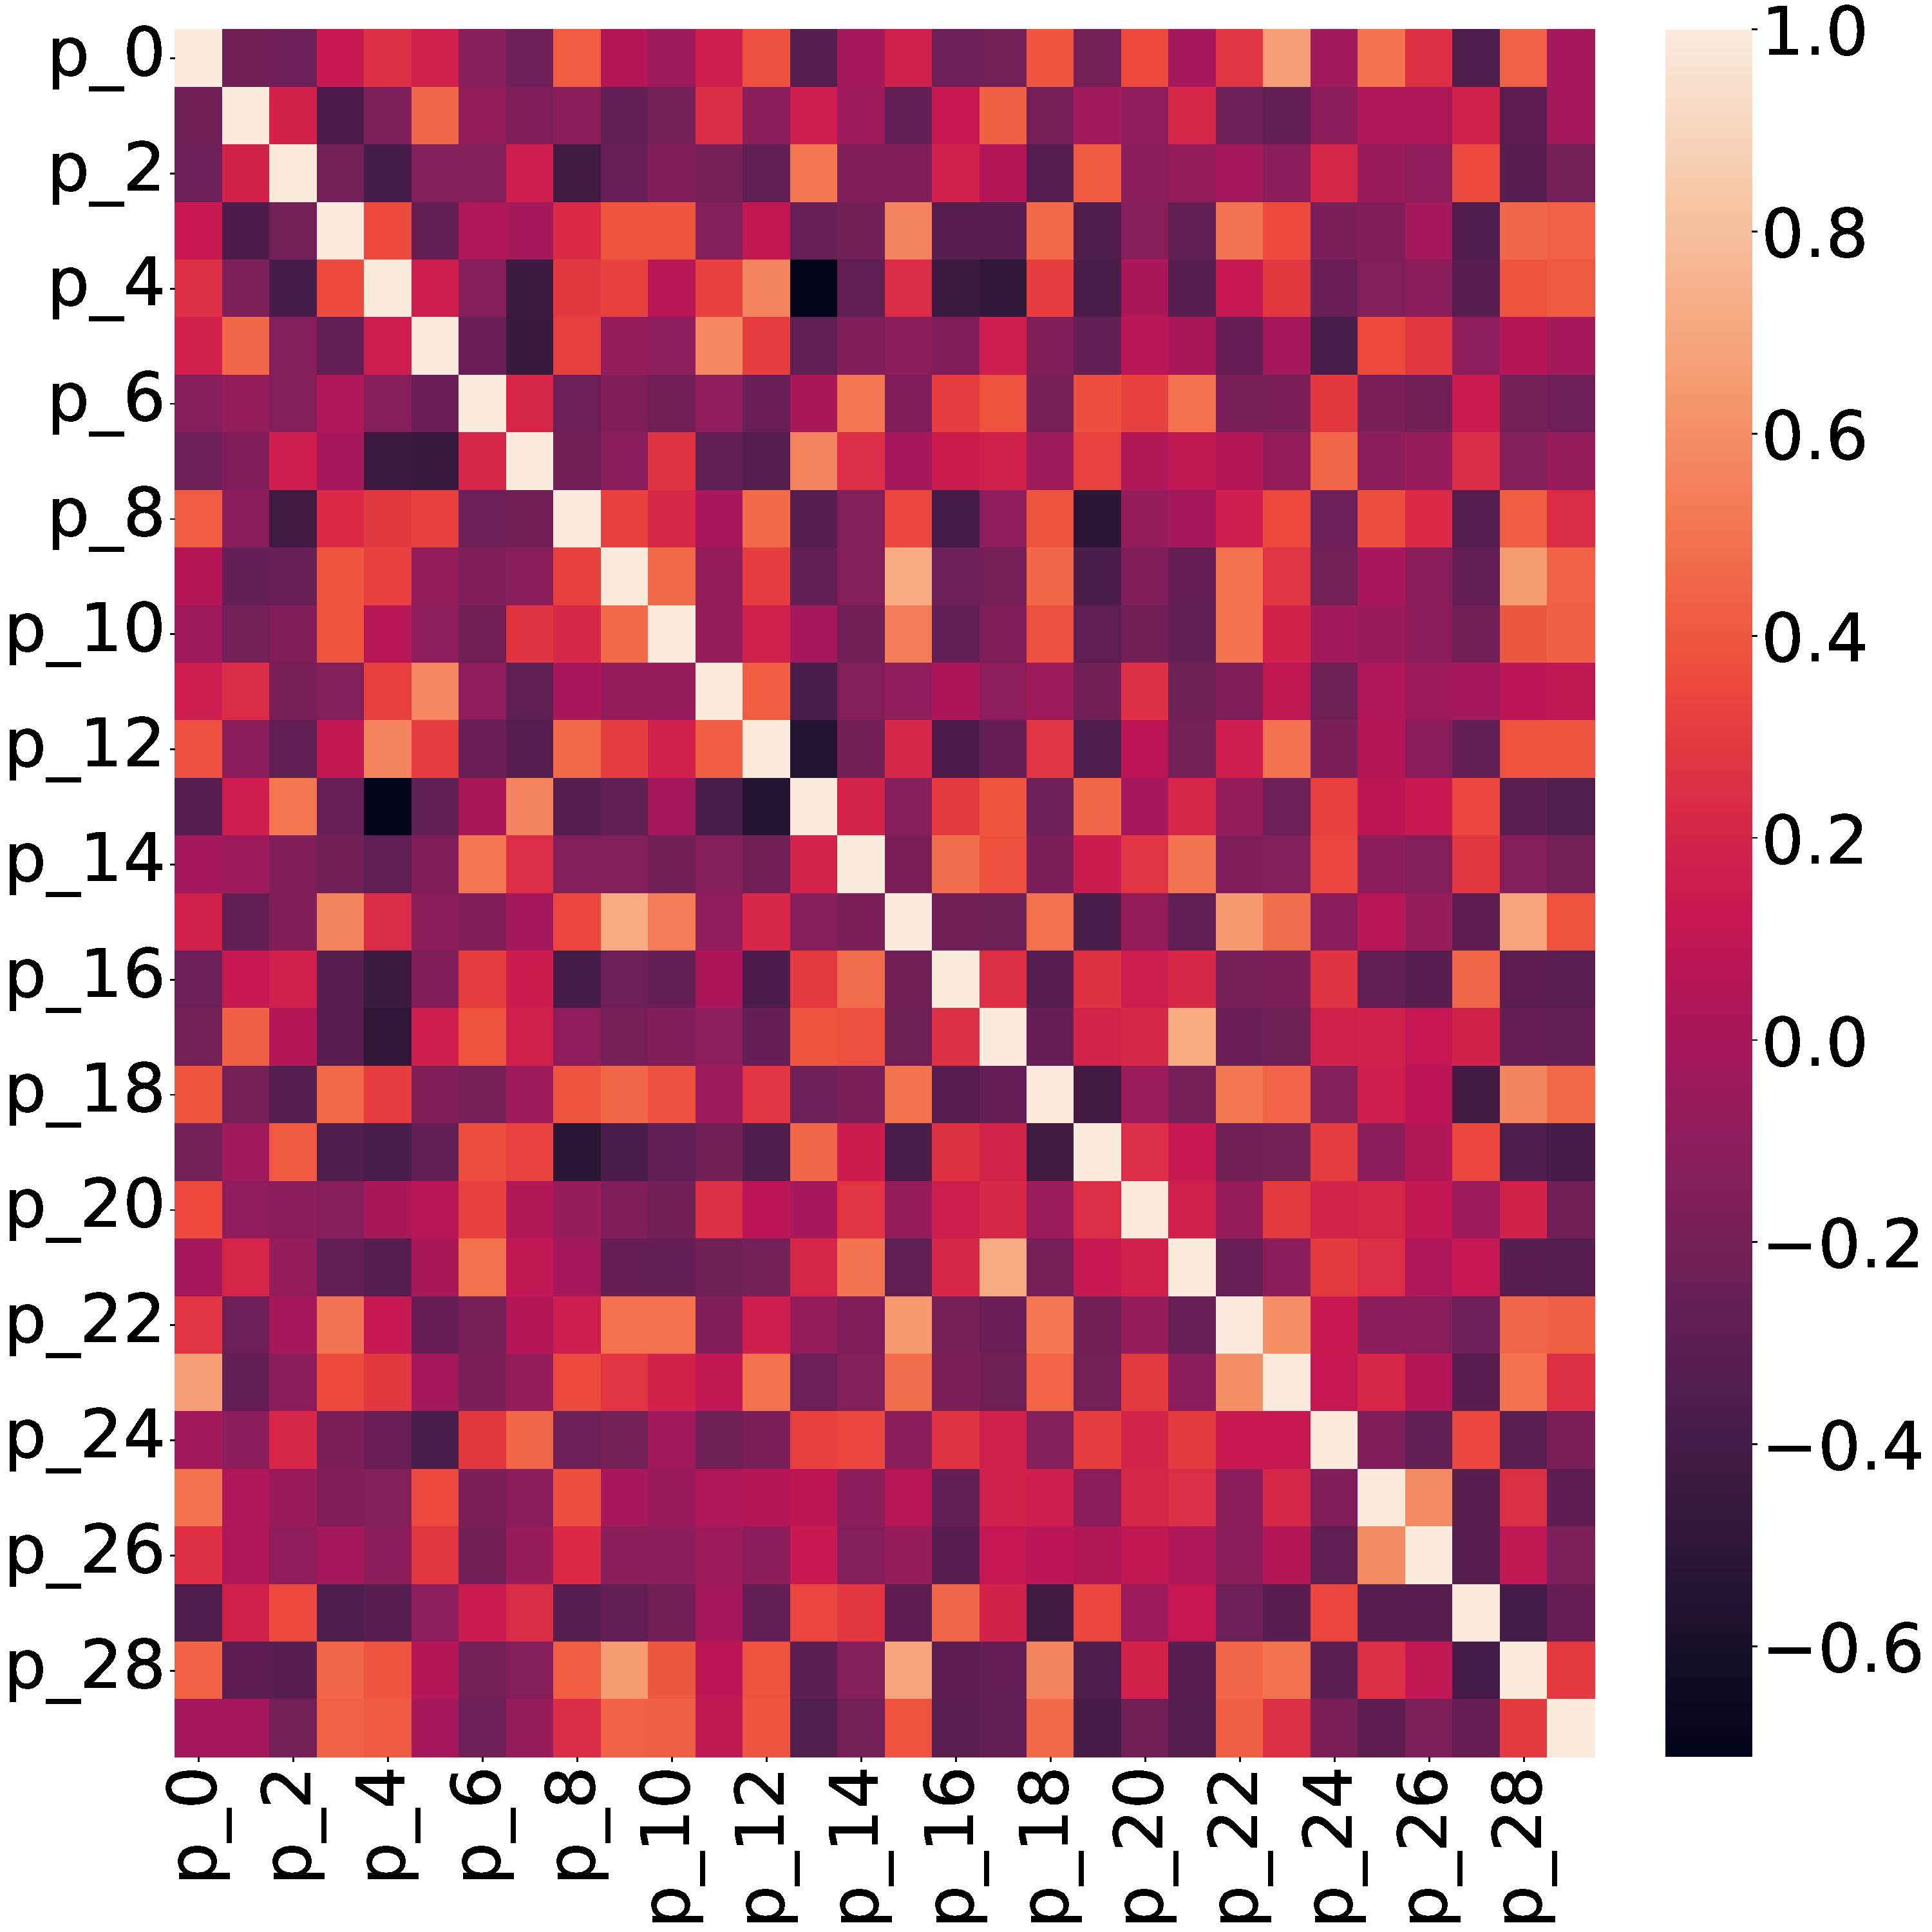
\includegraphics[width=\textwidth]{imgs/cem/KANDY_2-vit-continual-triplet_pp.pdf}
		\caption{Triplet loss}
	\end{subfigure}
\end{minipage}
\hfill
\begin{minipage}{.49\textwidth}
	\centering
	{\small\sc Discovered Concepts (rows)\\vs.\\Ground Truth Concepts (cols)}\\
\begin{subfigure}{.49\textwidth}
	%\hskip -2mm    
	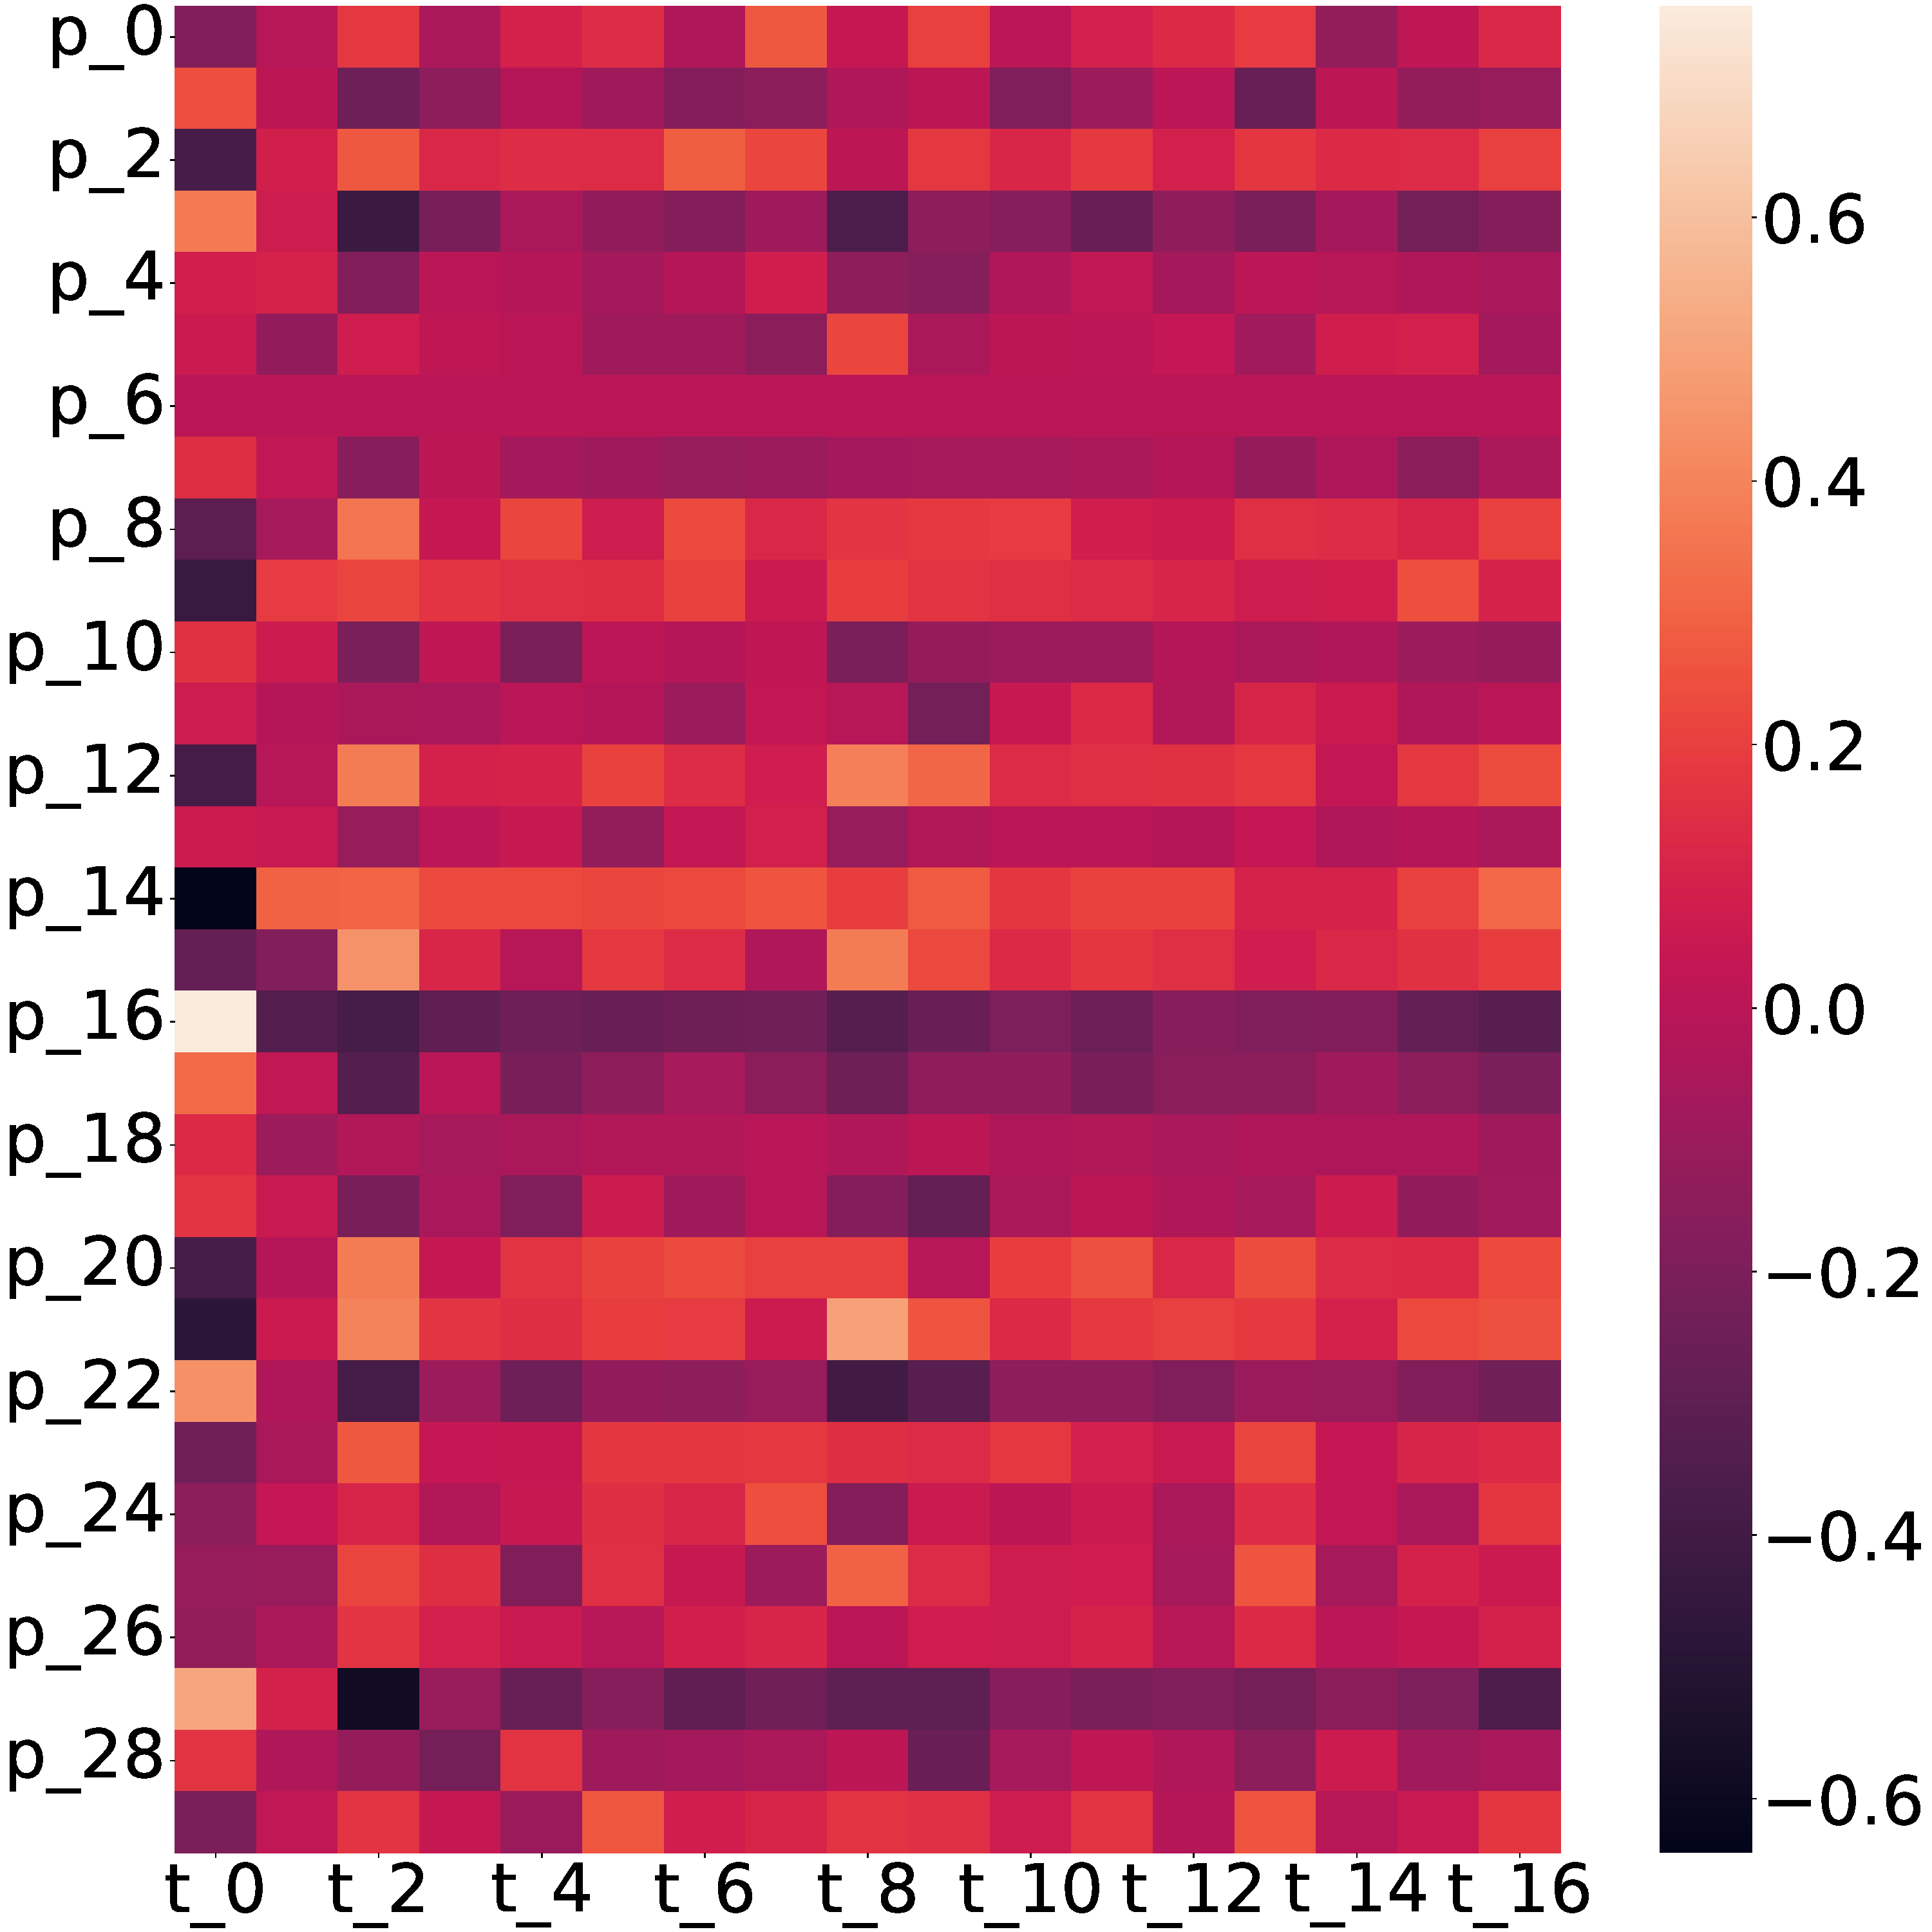
\includegraphics[width=\textwidth]{imgs/cem/KANDY_2-vit-continual-notriplet_pt.pdf}
	\caption{Simple}
\end{subfigure}
\begin{subfigure}{.49\textwidth}
	%\hskip -2mm    
	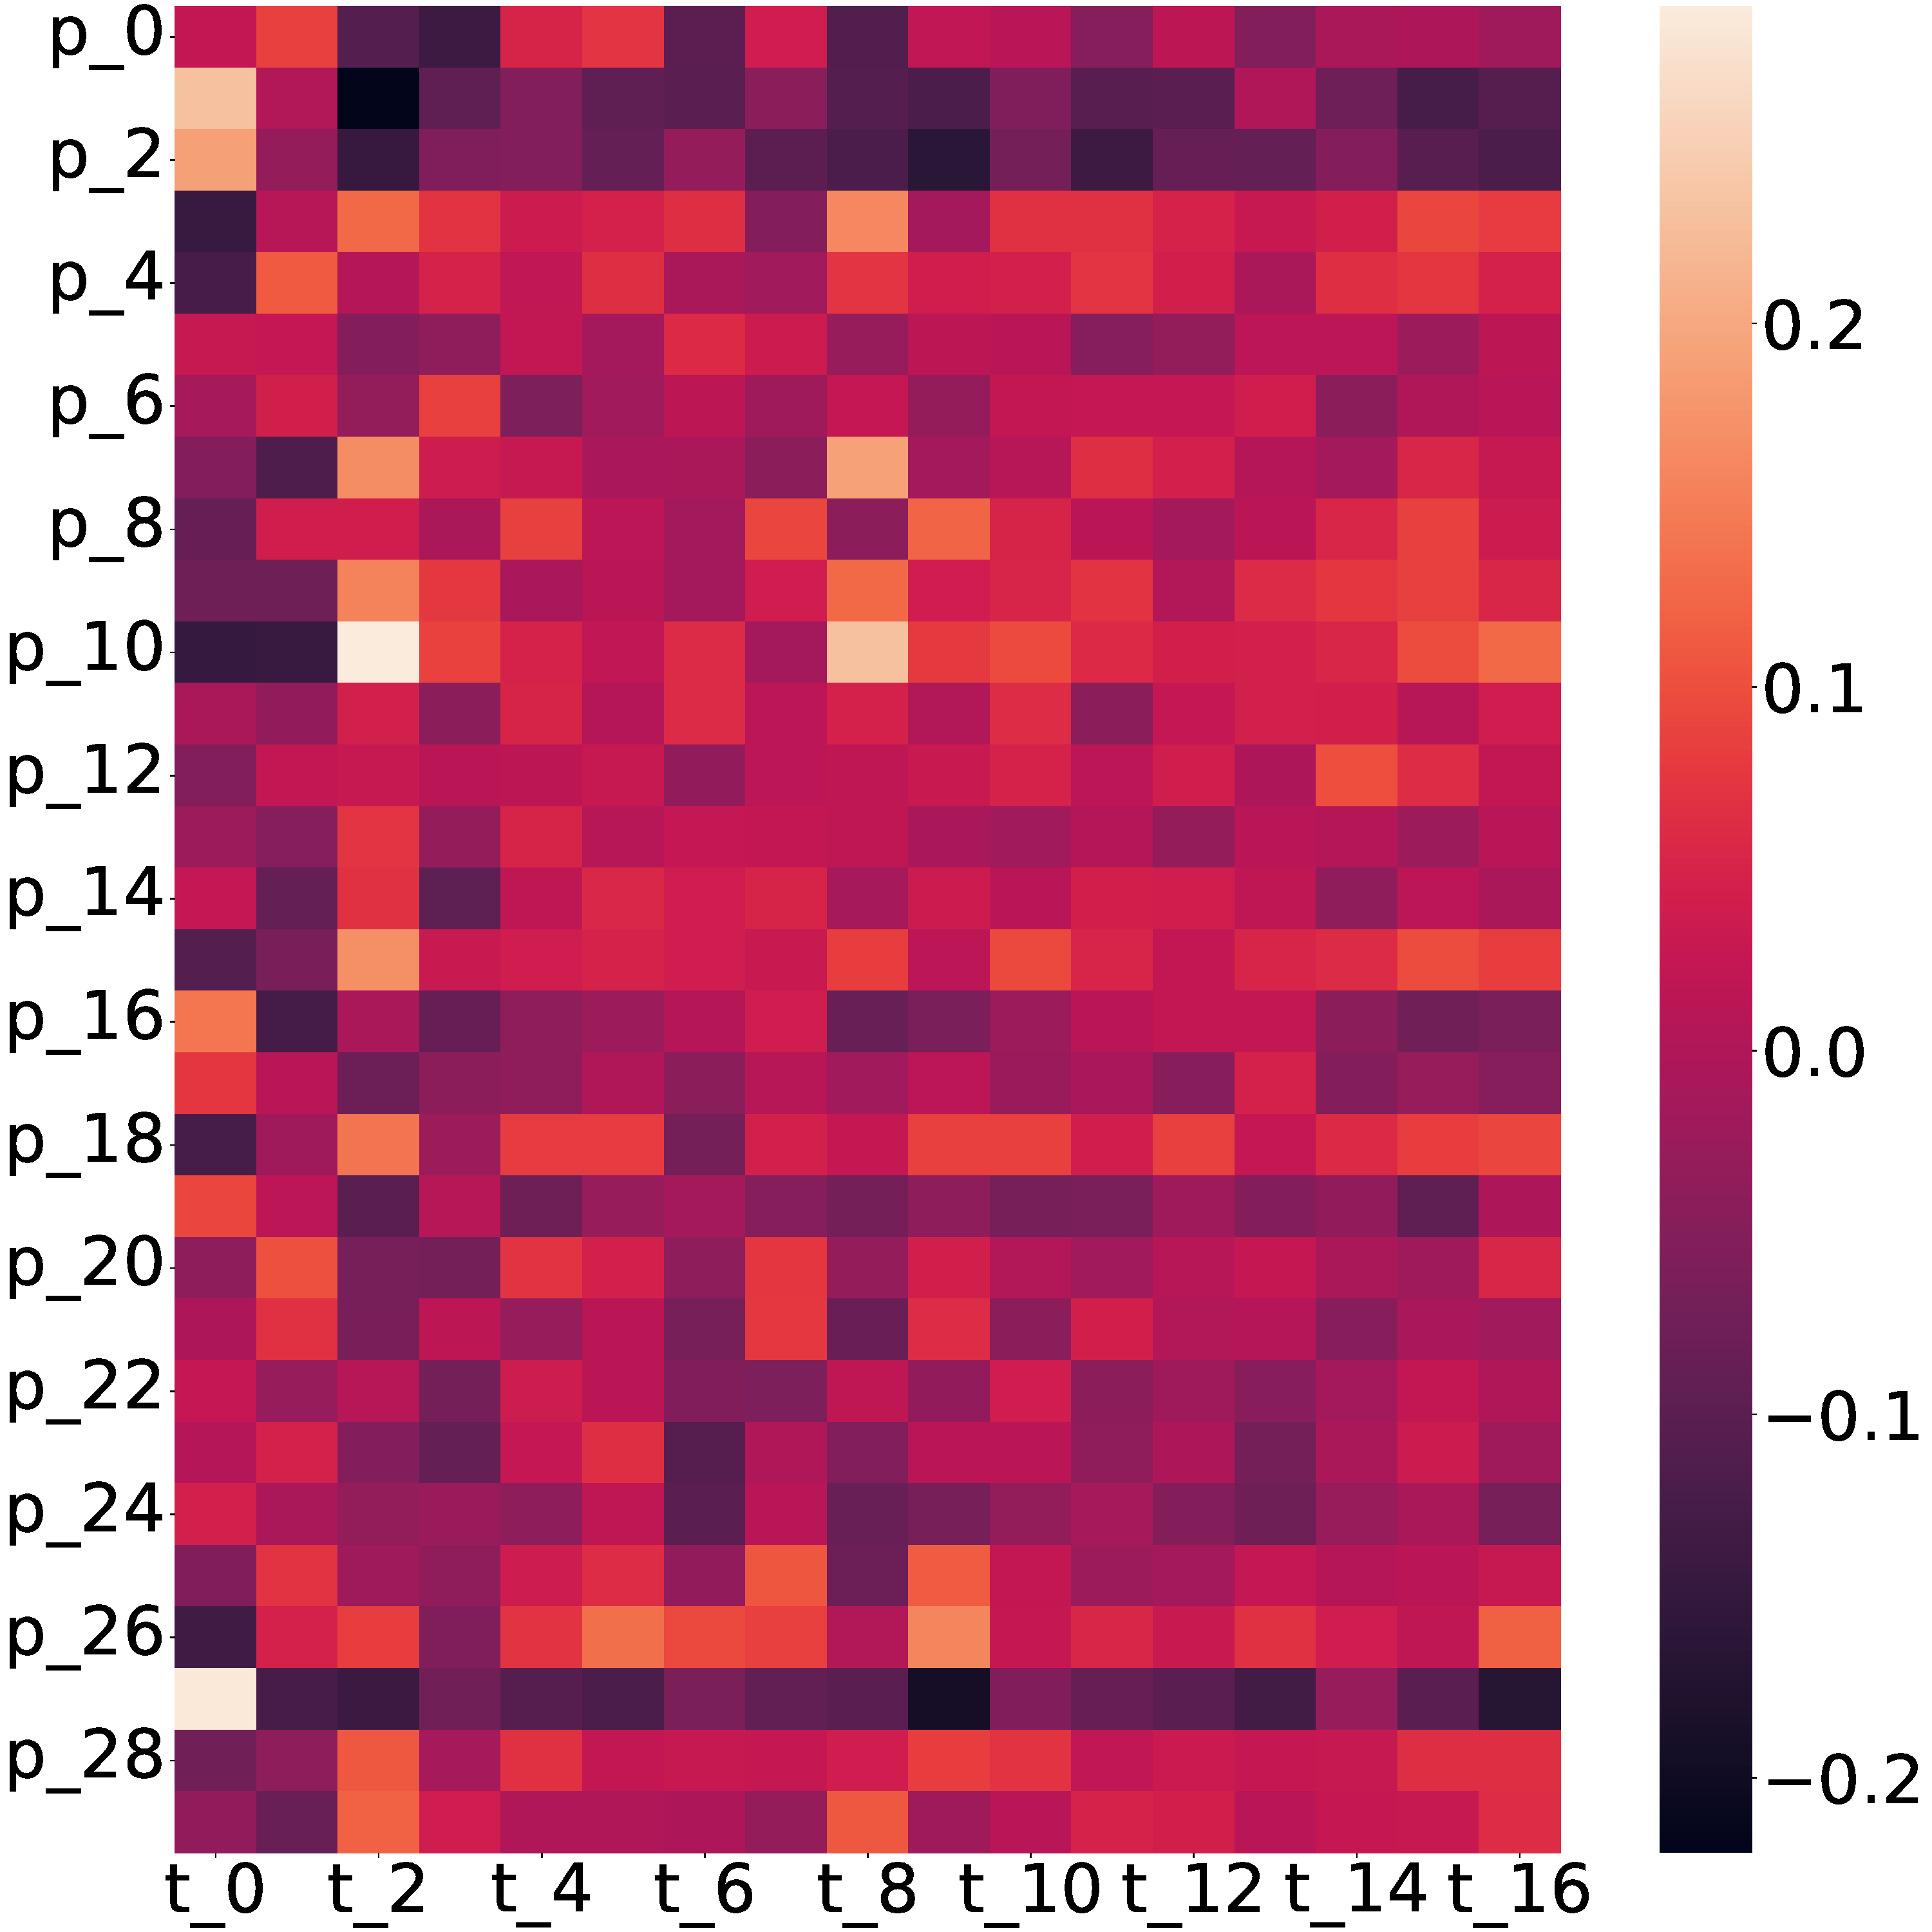
\includegraphics[width=\textwidth]{imgs/cem/KANDY_2-vit-continual-triplet_pt.pdf}
	\caption{Triplet loss}
\end{subfigure}
\end{minipage}
 
\caption[Concept correlation matrices for \textsc{KANDY-Concepts-2} (ViT-16)]{Correlation matrices computed via {\small\sc MCC}. Left (a,b): Learned concepts vs. themselves. Right (c,d): Learned vs. ground truth concepts. Triplet loss is active only in (b) and (d). Results regard ViT-16 model in the \textsc{KANDY-Concepts-2} dataset.
%\vspace{-4mm}
}
\label{cem:fig:mcc}
\end{figure}
